\documentclass[type=master,fontset=fandol]{thuthesis}
% 选项:
%   type=[bachelor|master|doctor|postdoctor], % 必选
%   fontset=[fandol|custom],                  % 字体选择
%   secret,                                   % 可选
%   pifootnote,                               % 可选(建议打开)
%   openany|openright,                        % 可选,基本不用
%   arial,                                    % 可选,基本不用
%   arialtoc,                                 % 可选,基本不用
%   arialtitle                                % 可选,基本不用

% **生僻字乱码的解决方法**
% 先解释一下原因: 自带的 fandol 字体不包含生僻字,常用的中易字体因为版权
% 原因不能在 overleaf 发布。
% 解决方法: 找一台 windows 电脑,从 C:\Windows\Fonts 里把
%   simsun.ttc simhei.ttf simkai.ttf simhei.ttf
% 复制出来,上传到 fonts 文件夹,再设置 typeset=custom 即可。


% 所有其它可能用到的包都统一放到这里了,可以根据自己的实际添加或者删除。
\usepackage{thuthesis}
\usepackage{amsmath}
\usepackage{pifont}% http://ctan.org/pkg/pifont
\newcommand{\cmark}{\ding{51}}%
\newcommand{\xmark}{\ding{55}}%
\newcommand{\tabincell}[2]{\begin{tabular}{@{}#1@{}}#2\end{tabular}} 
% 定义所有的图片文件在 figures 子目录下
\graphicspath{{figures/}}
\usepackage{listings}
\usepackage{xcolor}

\lstset{
    %backgroundcolor=\color{red!50!green!50!blue!50},%代码块背景色为浅灰色
    rulesepcolor= \color{gray}, %代码块边框颜色
    breaklines=true,  %代码过长则换行
    numbers=left, %行号在左侧显示
    numberstyle= \small,%行号字体
    %keywordstyle= \color{blue},%关键字颜色
    commentstyle=\color{gray}, %注释颜色
    frame=shadowbox%用方框框住代码块
    }
% --------------------- 
% 作者:da_kao_la 
% 来源:CSDN 
% 原文:https://blog.csdn.net/da_kao_la/article/details/83105948 
% 版权声明:本文为博主原创文章,转载请附上博文链接!
% 可以在这里修改配置文件中的定义。导言区可以使用中文。
% \def\myname{薛瑞尼}

\begin{document}

%%% 封面部分
\frontmatter
\thusetup{
  %******************************
  % 注意:
  %   1. 配置里面不要出现空行
  %   2. 不需要的配置信息可以删除
  %******************************
  %
  %=====
  % 秘级
  %=====
  secretlevel={公开},
  secretyear={19},
  %
  %=========
  % 中文信息
  %=========
  ctitle={基于方面的情感分析及其\\在新闻驱动的股票预测中的应用},
  cdegree={工学硕士},
  cdepartment={计算机科学与技术系},
  cmajor={计算机科学与技术},
  cauthor={潘寅旭},
  csupervisor={宋斌恒 副教授},
%   cassosupervisor={陈文光教授}, % 副指导老师
%   ccosupervisor={某某某教授}, % 联合指导老师
  % 日期自动使用当前时间,若需指定按如下方式修改:
  % cdate={超新星纪元},
  %
  % 博士后专有部分
  cfirstdiscipline={计算机科学与技术},
  cseconddiscipline={系统结构},
  postdoctordate={2016年7月——2019年7月},
  id={编号}, % 可以留空: id={},
  udc={UDC}, % 可以留空
  catalognumber={分类号}, % 可以留空
  %
  %=========
  % 英文信息
  %=========
  etitle={Aspect-based Sentiment Analysis for News-driven Stock Prediction},
  % 这块比较复杂,需要分情况讨论:
  % 1. 学术型硕士
  %    edegree:必须为Master of Arts或Master of Science(注意大小写)
  %             “哲学、文学、历史学、法学、教育学、艺术学门类,公共管理学科
  %              填写Master of Arts,其它填写Master of Science”
  %    emajor:“获得一级学科授权的学科填写一级学科名称,其它填写二级学科名称”
  % 2. 专业型硕士
  %    edegree:“填写专业学位英文名称全称”
  %    emajor:“工程硕士填写工程领域,其它专业学位不填写此项”
  % 3. 学术型博士
  %    edegree:Doctor of Philosophy(注意大小写)
  %    emajor:“获得一级学科授权的学科填写一级学科名称,其它填写二级学科名称”
  % 4. 专业型博士
  %    edegree:“填写专业学位英文名称全称”
  %    emajor:不填写此项
  edegree={Master of Science},
  emajor={Computer Science and Technology},
  eauthor={Pan Yinxu},
  esupervisor={Associate Professor Song Binheng},
%   eassosupervisor={Chen Wenguang},
  % 日期自动生成,若需指定按如下方式修改:
  % edate={December, 2005}
  %
  % 关键词用“英文逗号”分割
%   ckeywords={\TeX, \LaTeX, CJK, 模板, 论文},
%   ekeywords={\TeX, \LaTeX, CJK, template, thesis}
}

% 定义中英文摘要和关键字
\begin{cabstract}
股票预测一直是学术界和商业界共同的研究热点之一。新闻事件能够影响交易员的决定,而股票价格的变动会被交易员的决定影响,因此,新闻事件是可以影响股票市场的。
之前的研究将文本挖掘的技术应用到股票预测当中,通过向量或结构化实体的方式来表示事件,忽视了新闻文本中的大量细节;同时,之前研究中用到的数据集大多是不公开的。
我们不再从新闻文本中提取事件表示,而是直接将新闻文本作为输入,为每支股票创建一个向量化的表示,并将股票预测转化为一个基于方面的情感分析问题,通过预测新闻对某支股票的影响,来预测股票价格的变动。我们构建了一个名为senti-stock的股票预测数据集。它包含约三万个样本,每个样本都是由来自路透社的新闻和来自雅虎财经的股票历史数据构建的。我们提出一个名为MSRMAM(基于注意力机制的多股票关系模型)的模型,它包括情感分析模块和股票关系模块。情感分析模块利用多尺度卷积和股票系数,多尺度卷积可以提取不同粒度的句子特征;股票相关系数是通过股票向量计算得到的,反映了股票相关的信息。股票关系模块利用了注意力机制,学习股票之间的相关关系。在senti-stock数据集上的实验结果证明了多股票关系模型的有效性。

本文的贡献点主要有:1)利用路透社的金融新闻和雅虎财经的股票历史数据,创建了新闻驱动的股票预测数据集senti-stock;2)提出了基于转换器和多尺度卷积的模型,用于对目标的情感分析;3)提出了股票向量的概念,并将新闻驱动的股票预测转化为基于方面的情感分析问题,提出了MSRMAM模型(基于注意力机制的多股票关系模型,Multi-Stock Relation Model using Attention Mechanism)用于新闻驱动的股票预测。


%   关键词是为了文献标引工作、用以表示全文主要内容信息的单词或术语。关键词不超过 5
%   个,每个关键词中间用分号分隔。(模板作者注:关键词分隔符不用考虑,模板会自动处
%   理。英文关键词同理。)
\end{cabstract}

% 如果习惯关键字跟在摘要文字后面,可以用直接命令来设置,如下:
\ckeywords{股票预测, 基于方面的情感分析, 多核卷积, 转换器}

\begin{eabstract}
  The stock market prediction has always been the hotspot research in academia and business. As news events affect human decisions and the volatility of stock prices is influenced by human trading, it is reasonable to say that news events can influence the stock market. Previous studies have applied text mining techniques to predict stock prices by using structured entities or dense vectors to represent news events. And most datasets used in previous studies are not publicly available. We take the news text as input, create an embedding vector for each stock, and regard news-driven stock prediction as an aspect-based sentiment analysis problem. We try to predict stock prices by evaluating the impact of news on stocks. We create a stock prediction dataset named senti-stock. The dataset consists of 30 thousand samples, which is made up of online financial news (from Reuters) and stock history price (from Yahoo Finance). We propose a model named MSRMAM (Multi-Stock Relation Model using Attention Mechanism), which consists of sentiment analysis module and stock relation module. The sentiment analysis module is based on multi-scale convolution neural network with stock coefficient. The multi-scale CNN can extract sentence features in different granularities. The stock coefficient, which is computed using the stock embedding is used to adjust the sentence features. The stock relation module uses attention mechanism to learn the relations between stocks. Experiments on the senti-stock dataset demonstrate the effectiveness of our model.
  
 
  The main contributions of this paper are:1)create a dataset named senti-stock using Reuters news and Yahoo Finance history data;2) propose a model using transformer and multi-scale CNN;3)  convert news-driven stock prediction to an aspect-based sentiment analysis problem by creating a vector for each stock and propose MSRMAM (Multi-Stock Relation Model using Attention Mechanism).
\end{eabstract}

\ekeywords{Stock Prediction, Aspect-based Sentiment Analysis, Multi-scale CNN, Transformer}

% 如果使用授权说明扫描页,将可选参数中指定为扫描得到的 PDF 文件名,例如:
% \makecover[scan-auth.pdf]
\makecover

%% 目录
\tableofcontents

%% 符号对照表
\begin{denotation}[3cm]
\item[CNN] 卷积神经网络 (Convolution Neural Network)
\item[RNN] 循环神经网络 (Recurrent Neural Network) 
\item[LSTM] 长短时记忆网络 (Long Short Term Memory Network)
\item[GRU] Gated Recurrent Unit
\item[ABSA] 基于方面的情感分析 (Aspect-based Sentiment Analysis)
\item[ACSA] 对某一方面的情感分析 (Aspect-Category Sentiment Analysis)
\item[ATSA] 对某一目标的情感分析 (Aspect-Term Sentiment Analysis)
\item[SVM] 支持向量机 (Support Vector Machine)
\item[Bag of Words] 词袋模型
\item[TFIDF] 词频与逆向文档频率 (Term Frequency Inverse Document Frequency)
\item[MSRA] 使用attention的多股票关系模型 (Multi-Stock Relation Model using Attention mechanism) 
\end{denotation}



%%% 正文部分
\mainmatter
\chapter{介绍}
\label{cha:introduction}

\section{研究内容}

股票(stock)是股份公司发行的所有权凭证,是股份公司为筹集资金而发行给各个股东作为持股凭证并借以取得股息和红利的一种有价证券。每股股票都代表股东对企业拥有一个基本单位的所有权。每家上市公司都会发行股票。股票趋势预测一直是股票投资所关注的热点之一,优秀的股票预测可以带来巨大的收益。因此,股票预测一直是学术界和金融界共同的研究兴趣。

大量经验性的研究表明,股票在某种程度上是可以被预测的。行业研究员通过基本面研究,由股票公司的运行情况、相关政策、新闻等,股票的估值进行预测;量化分析师通过技术分析,运用数学、统计的方法,从股票历史交易数据中,寻找规律,进行股票趋势预测。而在本文中,我们专注于解决新闻驱动的股票预测问题。新闻事件能够影响交易员的决定,交易员的交易影响股票的价格。因此,我们可以认为,新闻事件是可以影响股票价格的。

随着自然语言处理技术的发展,使用人工智能的方法处理新闻文本,提取相关信息成为了可能。我们提出为每个股票创建一个相应的向量,从而将新闻驱动的股票预测转化为了基于方面的情感分析(其目标是提取句子对某一方面或目标的情感极性)。我们假设股票的涨跌仅受前一个时间段的新闻的影响,通过预测新闻(文本)对股票(目标)的影响(情感极性),来预测股票的涨跌。
\section{研究背景}

近期的研究工作开始应用文本挖掘技术分析新闻对股票市场的影响。研究者使用OpinionFinder~\cite{Wilson2005OpinionFinder}和Google-Profile of Mood States (GPOMS)工具,来研究推特(Twitter)情绪是否会影响道琼指数(Dow Jones Industrial Average, DJIA)\cite{bollen2011twitter}。他们利用上述两款工具处理推特数据,获取了情绪的时间序列,并以此预测道琼指数的每日涨跌,获得了87.6\%的准确率。这一研究表明,网络内容的情感信息与股票市场的变动是相关的。之后,有研究者提出了结构化的事件表示方法\cite{ding2014using}。他们提出使用信息抽取的方法来得到事件的表示,在不使用人力的情况下,从大规模的公开新闻中得到事件的结构化表示,即一个包括主语、谓语、动作和时间的四元组。他们利用线性和非线性的模型,探索新闻事件和股票市场之间的隐含的复杂关系。他们预测标普500的变化的准确率达到了60\%,预测单支股票的准确率超过了70\%。为进一步提升事件驱动的股票预测的准确率,优化事件的表示形式,又有研究者用深度学习的方式来解决这一问题\cite{ding2015deep}。首先,他们从新闻文本中提取事件,用一个向量表示事件,并用一个神经网络对其进行训练;然后,用一个深度卷积网络来预测股票的短期和长期变化。相比于之前的方法,他们将预测标普500和单支股票涨跌的准确率提升了将近6\%。

上述研究工作主要存在两个问题:首先,他们利用词袋模型、结构化四元组、稠密向量的方式来表示事件,随着自然语言处理技术的发展,这些表示方式已经不是新闻事件的最优化表示方式了;然后,这些工作中所用到的数据集大都是不公开的,影响了进一步的后续研究。

\section{本文贡献}

为解决第一个问题,我们利用自然语言处理的技术,直接将新闻文本作为事件输入。同时,我们提出为每一个股票创建一个向量表示,即股票向量的概念。据我们所知,这是第一次提出股票向量的概念。这样,我们将新闻驱动的股票预测转化为预测新闻事件对某支股票的影响。这一问题在自然语言处理中,被称为基于方面的情感分析,其目标是预测一段文本(新闻文本)对某一特定方面(股票)或目标的影响(涨跌)。比如,“微软收购诺基亚手机部门”这一新闻对微软来说是积极的,将会导致微软的股票在下一个时间段内上涨;对诺基亚来说是消极的,将导致诺基亚的股票在下一时间段内下跌。

为解决第二个问题,我们创建了一个新闻驱动的股票预测的数据集。我们从互联网的公开数据中抓取原始数据。利用来自于路透社的新闻数据,以及来自于雅虎财经的股票历史数据,我们构建了名为senti-stock的数据集。在这里,我们假设股票价格的涨跌仅与股票在前一个时间段(前一天、周、月)的相关新闻有关,忽略其他的影响因素。我们将新闻文本以及与这条新闻相关的股票作为输入,将股票在下一个时间段(日、周、月)内的变动情况作为输出标签。具体地,如果股票在下一个时间段内(日、周、月)的涨幅超过1\%,则将输出标签设为$+1$,如果股票在下一个时间段(日、周、月)的跌幅超过1\%,则将输出标签设为$-1$,其他的输出标签设为$0$。

为解决基于方面的情感分析问题,并将其应用于股票预测,我们提出了自己的模型。

首先,为解决LSTM的无法并行化的缺陷和CNN不擅长解决长期依赖的问题,我们提出使用transformer~\cite{NIPS2017_7181}和多尺度卷积的模型来解决基于方面的情感分析问题。Transformer的结构由谷歌提出,它完全抛弃了LSTM和CNN,仅使用self-attention就在自然语言处理的诸多应用中取得了优秀的结果,可以处理长期依赖问题,并且便于并行化。多尺度卷积利用了全部单词的表示,从不同的粒度提取了特征。我们的这一模型,在三个公开数据集Restaurant、Laptop、Twitter上取得了最佳的结果。

然后,为了在senti-stock这一数据集上取得更好的结果,我们提出了基于attention机制的股票关系模型MSRA(使用attention机制的多股票关系模型, Multi-Stock Relation model using Attention mechanism)。MSRA包括了情感分析模块和股票关系模块。情感分析模块使用多尺度卷积来学习新闻文本的特征。同时,为了考虑股票的相关信息,我们引入了股票系数。股票系数由股票向量通过一个全连接层学习得到,它引入了股票的相关信息。另外,股票之间的相互关系也对股票的变化有着巨大的影响。我们引入了attention机制,利用attention机制学习得到股票之间的相互关系。MSRA在senti-stock数据集上取得了最佳的结果。

% Please add the following required packages to your document preamble:
% \usepackage{multirow}
\begin{table}[ht]
	\centering 
	\caption{基于方面的情感分析主要研究内容}
	\label{tab:content}
	\begin{tabular}{|l|l|l|l|}
	\hline
	任务                                               & 应用场景                  & 数据集         & 模型                                 \\ \hline
	\multirow{3}{*}{ATSA} & \multirow{2}{*}{评论分析} & Restaurant  & \multirow{3}{*}{\textbf{Transformer\&MCNN}} \\ \cline{3-3}
													 &                       & Laptop      &                                    \\ \cline{2-3}
													 & 社交媒体分析                & Twitter     &                                    \\ \hline
	ACSA               & \textbf{股票预测}                  & \textbf{senti-stock} & \textbf{MSRA}                               \\ \hline
	\end{tabular}
\end{table}

表~\ref{tab:content}显示了基于方面的情感分析的主要研究内容。基于方面的情感分析(Aspect-based Sentiment Analysis)旨在提取句子对某一方面或目标的情感极性,又可以细分为对某一目标的情感分析(Aspect-Term Sentiment Analysis, ATSA)和对某一方面的情感分析(Aspect-Category Sentiment Analysis, ACSA)。二者都是一种更细化的情感分析任务,不同的是,对某一目标的情感分析希望提取句子对某一目标的情感极性,这里的目标必须是在句子中出现的一个子串;而对某一方面的情感分析希望提取句子对某一方面的情感极性,这里的方面,并不一定出现在句子当中,而是与句子内容相关的某一方面。比如,“比萨很好吃!”这一句子,对目标“比萨”的情感极性是积极的,对方面“味道”的情感是积极的,“比萨”是出现在句子中的一个子串,而“味道”是与句子内容相关的某一方面,并不一定在句子中出现。在对某一目标的情感分析中,我们提出了使用transformer和多尺度卷积的模型;我们还将对某一方面的情感分析应用于股票预测,构建了senti-stock数据集,提出了MSRA基于attention机制的多股票关系模型。除此之外,我们还调研了大量的文献,总结了新闻驱动的股票预测和基于方面的情感分析之前的研究工作,并复现了多个之前基于方面的情感分析的模型,并将这些模型的实现开源。表格中加粗的部分是我们的主要工作。

  本文的贡献点主要有:
\begin{itemize}
	\item 我们利用路透社的金融新闻和雅虎财经的股票历史数据,创建了新闻驱动的股票预测数据集;
	\item 我们提出了股票向量的概念,并将新闻驱动的股票预测转化为基于方面的情感分析问题;
	\item 提出了基于transformer和多尺度卷积的模型,并在多个开放数据集上取得了最佳的实验效果;
	\item 提出了MSRA模型(使用attention机制的多股票关系模型,Multi-Stock Relation model using Attention mechanism),并在senti-stock数据集上取得了最佳的效果。
\end{itemize}

\section{组织结构}

本文研究基于方面的情感分析及其在新闻驱动的股票预测中的应用\footnote{由于字母符号数量限制,本文中各章节的字母符号可能表示不同的含义,相互不冲突。}。第一章介绍了全文的主要内容;第二章介绍新闻驱动的股票预测和基于方面的情感分析的相关工作;第三章介绍我们所用到的数据集,包括开放数据集Reataurant、Laptop、Twitter,以及我们所创建的新闻驱动的股票预测数据集senti-stock;第四章,我们介绍用于对目标情感分析的模型,使用了transformer结构和多尺度卷积;第五章,我们介绍用于新闻驱动的股票预测模型,提出股票向量的概念,使用了多尺度卷积,利用股票系数来调整句子特征,并利用attention机制学习股票之间的相关关系;第六章介绍了我们的实验设置以及实验结果,我们的模型在公开数据集和股票预测数据集上分别取得了最佳的结果;最后,我们在第七章总结本文的内容。
\chapter{相关工作}
\label{cha:relatedwork}

股票预测一直是股票投资所关注的一个重点,成功的预测可以为投资者创造巨大的收益。通过人工智能的方法,对股票涨跌进行预测,成为了计算机与金融的交叉领域的研究热点之一。在本章中,我们将介绍股票市场相关知识、新闻事件驱动的股票市场预测和基于方面的情感分析的相关工作。
\section{股票市场相关知识}
股票能否被预测一直是一个值得讨论的话题,在这些讨论中,有效市场假说是非常重要的一个理论。有效市场假说(Efficient Market Hypothesis,简称EMH)是由尤金法玛于1970年整理提出的\cite{fama1970efficient}。这一研究起源于路易斯巴舍利,他使用随机过程的方法,研究股票价格变化的随机性和布郎运动,他认为,过去、现在和未来的事件都 反映在股票市场的价格当中,股价遵循公平游戏模型。尤金法玛总结了前人的理论和实证,提出了有效市场假说,包括以下三个要点。
\begin{itemize}
    \item 市场中每个人都是理性的,市场中每支股票都处于这些理性人的监视之下,他们每天对股票价格进行分析和预测,并谨慎地在风险与收益之间进行取舍;
    \item 股票价格反映了这些理性人的供求平衡,买方等于卖方;
    \item 股票的价格反映了全部的可获取信息,当有新的消息出现时,股票价格会迅速地调整到合理的价位。
\end{itemize}
有效市场假说意味着“天下没有免费的午餐”,人们无法在有效市场中获得超额收益。然后有效市场假说也不一定完全正确,不是每个交易者都是完全的理性人,信息也并不一定在每个时刻都发生效果。有效市场假说被越来越多地证明不符合现实。

有效市场假说面临许多理论挑战:
\begin{itemize}
	\item 投资者并非完全理性的;
	\item 投资者不仅偶然偏离理性,而是经常以同样的方式偏离理性;
	\item 套利者不会完全消除非理性投资者的错误对价格的影响。
\end{itemize}
随着人工智能技术的发展,之前的研究表明,股票价格在某种程度上是可以被预测的。
\begin{figure}[ht]
	\centering 
	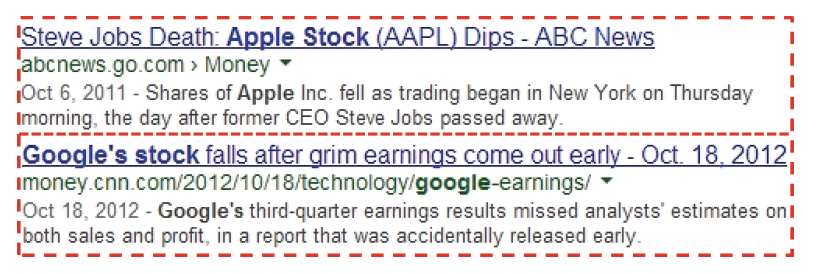
\includegraphics[width=0.8\linewidth]{NEWS-EVENT.png}
	\caption{苹果公司和谷歌公司相关新闻两则}
	\label{fig:stock-event}
\end{figure}
如图\ref{fig:stock-event}显示了两条金融新闻。在苹果前CEO乔布斯去世后,苹果的股票价格开始下跌;同时,在谷歌的收入报告公布后,由于收入不理想,谷歌的价格开始下跌。从中可以看出,新闻事件对股票市场有着重要的影响。
%另一方面,分型市场假说(Fractal Market Hypothesis,简称FMH),建立在非线性动力系统之上,利用流动性和投资起点很好地解释了有效市场假说无法理解的市场现象。分形市场假说主要内容包括:
%\begin{itemize}
%    \item 市场中有许多水平不同的投资者,投资者水平不同会对其行为产生重大影响;
%    \item 信息对不同水平的投资者影响不同,频繁交易的交易员会更加关注技术分析信息。而市场中基本分析投资者更关注对股票价格进行价值评估。在分型市场假说中,技术分析和基本分析都适用,但其影响与投资者的水平相关;
%    \item 市场稳定在于流动性的保持,只有市场处在不同投资水平的众多投资者组成时,流动性才能得以实现;
%    \item 价格反映了市场中的基于技术分析的短期评估和基于基本分析的价值评估;
%    \item 如果股票市场与整体经济循环无关,则市场本身并无长期趋势可言,交易、流动性和短期信息将在市场中起决定作用。
%\end{itemize}
%与有效市场假说不同的是,分形市场假说认为信息的重要性是按照不同投资者来判断的。不同投资者对信息的判断不同,信息的传播并非均匀扩散的。价格并不能反映全部己有的信息,只是反映 与投资者相对应的信息的重要性。有效市场是分形市场的一个特例,分形市场假说拓展了有效市场的含义,更广泛、准确地刻画了市场。
% \begin{table}[ht]
%     \centering
%     \caption{有效市场假说和分形市场假说的对比}
%     \label{tab:compare}
%     \begin{tabular}{|l|l|l|}
%         \hline 
%         特征 & 有效市场理论 & 分形市场理论  \\ 
%         市场特征 & 线性孤立系统 & 非线性、开放、耗散系统 \\ 
%         均衡状态 & 均衡 & 允许非均衡 \\ 
%         系统复杂性 & 简单系统 & 具有分形、混沌等特性的复杂系统 \\ 
%         反馈机制 & 无反馈 & 正反馈 \\ 
%         对信息的反应 & 线性因果关系 & 非线性因果关系 \\ 

%     \end{tabular}
% \end{table}
\section{新闻驱动的股票预测}

股票市场能否被预测一直都是一个值得讨论的问题。大量经验性的研究表明,股价是可以被预测的~\cite{bollen2011twitter,ding2014using,ding2015deep,ding2016knowledge-driven}。新闻事件能够影响交易员的决定,而交易员的交易会影响股票的价格。因此,新闻事件可以影响股票价格的变动。

\subsection{推特情绪预测指数涨跌}
依照行为金融学的观点,情绪可以影响个体的行为和决定。为验证这一规律是否能扩展到大规模群体上,研究者研究了大规模的推特情绪状态与道琼指数(Dow Jones Industrial Average, DJIA)的相关性~\cite{bollen2011twitter}。他们使用两种情绪分析工具来分析每天推特的文本内容:OpinionFinder~\cite{Wilson2005OpinionFinder}和GPOMS(Google-Profile of Mood States)~\cite{Spielberger1972Profile}。

\subsubsection{OpinionFinder}
OpinionFinder是一个公开的软件工具\footnote{http://mpqa.cs.pitt.edu/opinionfinder/opinionfinder\_2/},用于提取句子级的主观情绪极性(积极或消极)。

预处理阶段,利用Standford提供的词性标注工具,对输入进行句子分割和词性标注;然后从中选取主观的能反应情绪的词语;然后基于朴素贝叶斯方法和情感词库,对文本进行分类。

\subsubsection{GPOMS}

GPOMS是原作者自己提出的一款情感分析工具,它使用了Profile of Mood States(POMS-bi),一个由严格审查的心理学仪器提供的词库。为了使这一词库可以应用于推特情绪的分析,作者对词库进行了扩充。推特内容的情感被细分为了六类,包括冷静(Calm),警惕( Alert),肯定( Sure),重要( Vital),和善( Kind)和高兴(Happy)。

利用上述两种工具,他们将推特情感分为六类,包括冷静(Calm),警惕( Alert),肯定( Sure),重要( Vital),和善( Kind)和高兴(Happy)。然后,他们利用格兰杰因果分析(Granger Causality Analysis)和自组织模糊神经网络(Self-Organizing Fuzzy Neural Network),来验证利用上述两种工具得到的情感时间序列是可以用来预测道琼指数的收盘价。他们预测道琼指数收盘价的涨跌的准确率达到了87.6\%。

这一研究表明,网络信息的情感极性是可以用来预测股票市场的变动的。

\subsection{结构化的事件表示}

为了解决新闻事件驱动的股票市场预测,研究者提出事件的结构化表示~\cite{ding2014using}。以往的新闻事件驱动的股票预测,往往使用浅层特征,比如词袋特征(Bag of Words),命名实体,名词等,无法获取实体关系信息。

他们提出结构化的事件表示,使用一个四元组$(O_1,P,O_2,T)$来表示事件,其中$P$表示动作(Action),$O_1$表示动作的发起者(Actor),$O_2$表示动作的作用者(Object),$T$表示动作发生的时间(Time)。比如,“2013年9月3日,微软同意以7.2亿美元的价格收购诺基亚的手机部门”这一新闻事件可以表示为(Actor=微软,Action=收购,Object=诺基亚手机部门,Time=2013年9月3日)。

具体地,研究者们使用依存关系分析器提取句子的结构,选取动词$P$(Action),然后将其左侧最近的名词作为动作的发起者$O_1$,将其右侧最近的名词作为动作的作用者$O_2$。下面我们简单介绍词袋特征和结构化的事件表示方法。

\subsubsection{词袋模型}

% 在信息检索中,词袋模型(Bag of Words Model)假定对于一个文本,忽略其词序和语法,句法,将其仅仅看做是一个词集合,或者说是词的一个组合,文本中每个词的出现都是独立的,不依赖于其他词是否出现,或者说当这篇文章的作者在任意一个位置选择一个词汇都不受前面句子的影响而独立选择的。
在这里,使用经典的TFIDF(Term Frequency–Inverse Document Frequency,词频与逆向文档频率)值作为词袋特征。TFIDF被用来评估某一字词对于一个文件集或一个语料库的重要程度。字词的重要性随着它在文件中出现的次数成正比增加,但同时会随着它在语料库中出现的频率成反比下降。

\subsubsection{结构化事件表示}

前面已经提到用一个四元组$(O_1,P,O_2,T)$来表示事件。为了解决数据稀疏性的问题,使用退化的特征,即使用元素的合并作为事件的表示,即$(O_1,P,O_2,O_1+P,P+O_2,O_1+P+O_2)$。具体地,对事件四元组(Microsoft,buy,Nokia's mobile phone business)可以表示为(\#arg1=Microsoft,\#arg2=buy,\#arg3=Nokia's mobile phone,\#arg4=Microsoft buy,\#arg5=buy Nokia's mobile phone business,\#arg6=Microsoft buy Nokia's mobile phone business)。然后,为每个字符串生成一个特定的向量表示,这几个字符串拼接起来作为事件的表示。因为动作、动作发起者、动作作用者的数据非常稀疏,这里去掉时态、复数等特征,并将动作转换为动作的类别,以减少数据的稀疏性。

同时,这里还使用了线性和非线性的模型来解决新闻事件驱动的股票预测问题。线性模型选取的是SVM(Supported Vector Machine,支持向量机)模型,非线性模型选取的是三层神经网络。

实验结果显示,预测标普500的准确率达到了60\%,单支股票预测的准确率超过70\%。

\subsection{深度学习与新闻驱动的股票预测}

前面所提到的结构化的事件表示方法,使用的是单词向量的拼接。为改进这一方法,研究者提出用一个神经网络来学习事件的表示。图~\ref{fig:neural-tensor-network}显示了提取事件特征所使用的网络结构。

\begin{figure}[ht]
    \centering 
    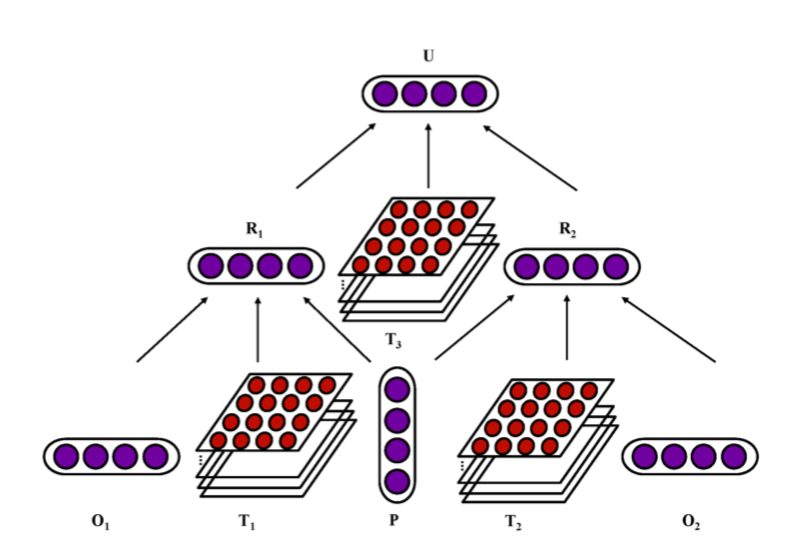
\includegraphics[width=0.5\linewidth]{neural-tensor-network.png}
    \caption{Neural Tensor Network结构}
    \label{fig:neural-tensor-network}
\end{figure}

这里用到的事件表示方法,与前面提到的四元组结构化表示一致。不同的是,不再使用退化的特征,而是使用一个神经网络Neural Tensor Network来训练学习得到事件的向量化表示。具体地,Actor、Action、Object均被表示为一个向量$O_1$、$P$、$O_2$。然后,利用矩阵$T_1$融合Actor~$O_1$和Action~$P$得到$R_1$,利用矩阵$T_2$融合Action~$P$和Object~$O_2$得到$R_2$,利用矩阵$T_3$融合$R_1$和$R_2$得到事件最终的向量表示。

模型上,这里用到了卷积神经网络。图~\ref{fig:cnn}显示了模型的结构。上面得到的事件的向量化表示被用来当作短期事件的表示,然后利用CNN和max pooling层得到中期和长期的事件表示。将短期、中期、长期的事件表示拼接起来,并通过两层神经网络预测得到最终的预测结果。

\begin{figure}[ht]
    \centering 
    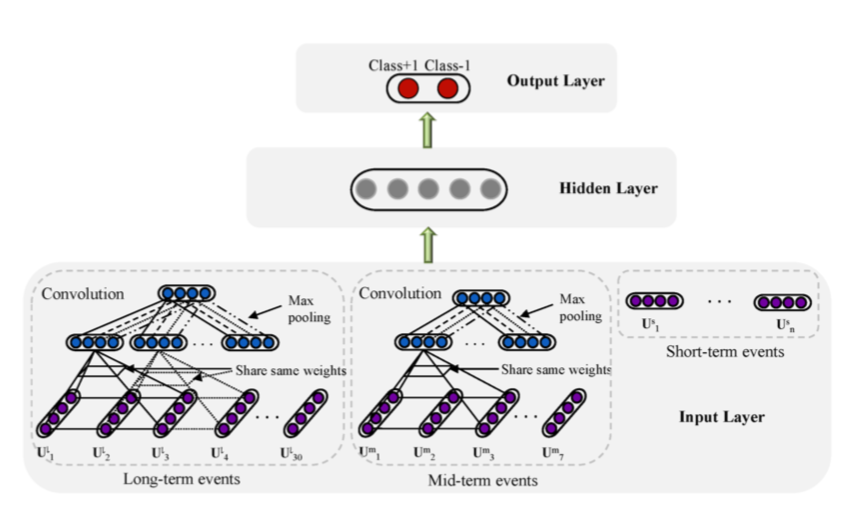
\includegraphics[width=0.5\linewidth]{CNN.png}
    \caption{基于CNN的预测模型结构}
    \label{fig:cnn}
\end{figure}

相比于之前的方法,利用神经网络学习得到的事件表示,可以将标普500的预测准确率提升将近6\%。

这些新闻事件驱动的股票预测表明,新闻事件与股票的变动是相关的,新闻事件可以用来作为股票预测的依据。但是,无论是利用OpinionFinder等工具的方法,还是结构化、向量化的表示,都忽视了新闻文本中的一些细节信息。随着自然语言处理技术的发展和词向量的提出,直接将新闻文本作为事件的表示,将股票预测转化为文本分类成为了更为合适的处理方式。

\section{基于方面的情感分析}

基于方面的情感分析旨在提取某个句子对某一方面或目标的情感极性~\cite{pontiki2014semeval-2014}。比如,“这家餐厅的菜很好吃,但服务太差了”对“食物”方面的情感是积极的,对“服务”方面的情感是消极的。基于方面的情感分析又细分为对某一方面的情感分析和对某一目标的情感分析。对某一方面的情感分析(Aspect-Category Sentiment Analysis)中,方面可能是一个抽象的概念,并不一定在句子当中出现;而对某一目标的情感分析(Aspect-Term Sentiment Analysis or Target-oriented Sentiment Analysis)中,目标一定是句子中的某一个词。随着自然语言处理技术的发展,研究者们提出了许多深度学习的模型来解决这一问题。

\subsection{ATAE-LSTM}

\begin{figure}[ht]
    \centering 
    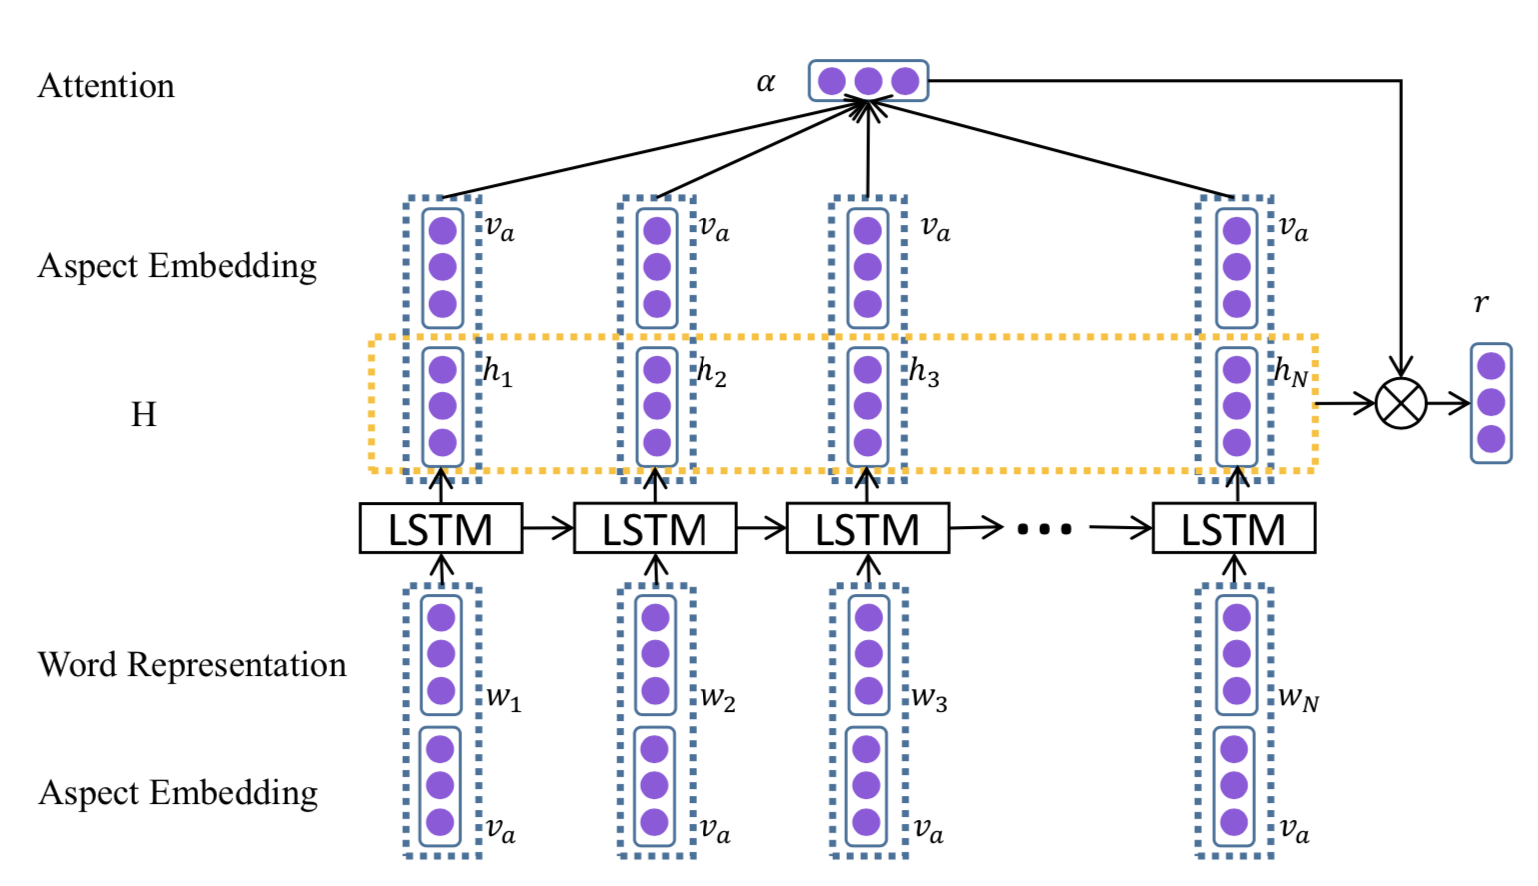
\includegraphics[width=0.8\linewidth]{atae-lstm.png}
    \caption{ATAE-LSTM模型结构}
    \label{fig:atae-lstm}
\end{figure}

ATAE-LSTM(Attention-based LSTM with Aspect Embedding)~\cite{wang2016attention-based}是一个结合了LSTM\cite{hochreiter1997long}和attention机制的模型。与直接使用LSTM模型相比,图~\ref{fig:atae-lstm}显示了ATAE-LSTM模型的结构。ATAE-LSTM使用了attention机制,当输入不同的aspect(方面)时,会对句子的不同部分有不同的侧重。因为aspect(方面)起着非常关键的作用,ATAE-LSTM模型用两种方式使用了aspect的信息:一个是在计算attention的加权和时,把aspect的信息和句子的隐式信息表示拼接起来;另一个是把aspect表示和输入单词向量拼接起来。ATAE-LSTM模型既可以处理对某一方面的情感分析(Aspect-Category Sentiment Analysis),也可以处理对某一目标的情感分析(Aspect-Term Sentiment Analysis or Target-oriented Sentiment Analysis)。ATAE-LSTM相比于LSTM模型,考虑了aspect的信息,引入了attention的机制。

\subsection{IAN}

\begin{figure}[ht]
    \centering
    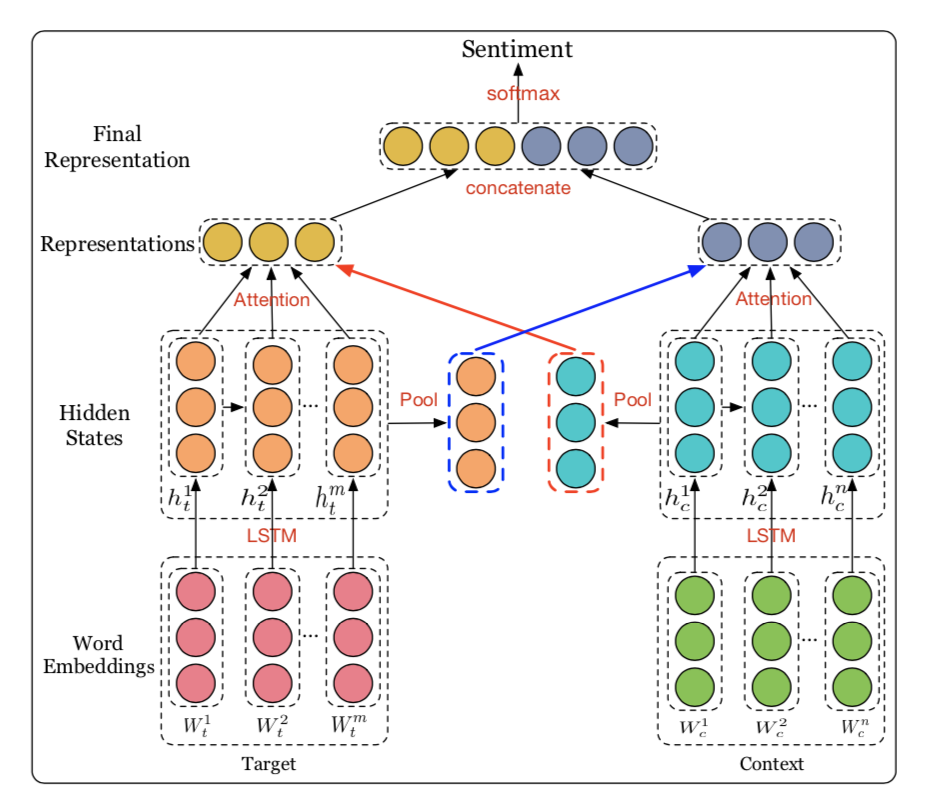
\includegraphics[width=0.7\linewidth]{ian.png}
    \caption{IAN模型结构}
    \label{fig:ian}
\end{figure}

在对某一目标的情感分析(Aspect-Term Sentiment Analysis or Target-oriented Sentiment Analysis)中,目标(target)可能由多个词组成。在针对不同的句子时,目标中的单词也可能发挥着不同的重要性。因此,IAN(Interactive Attention Networks)~\cite{ma2017interactive}提出目标的表示和句子的表示都需要通过交互式地学习得到。图~\ref{fig:ian}显示了IAN模型的结构。

首先,IAN使用LSTM处理句子和目标,得到了句子和目标的隐式向量表示。然后,通过均值pooling的方式,得到句子和目标的表示,并以此计算attention的权重,对句子和目标中的隐式表示进行加权求和。最后,将句子和目标的加权和结果拼接,作为整个输入的表示。IAN相比于ATAE-LSTM,使用了交互式的attention机制,同样考虑了目标中不同单词的不同重要性。

\subsection{BILSTM-ATT-G}

\begin{figure}[ht]
    \centering 
    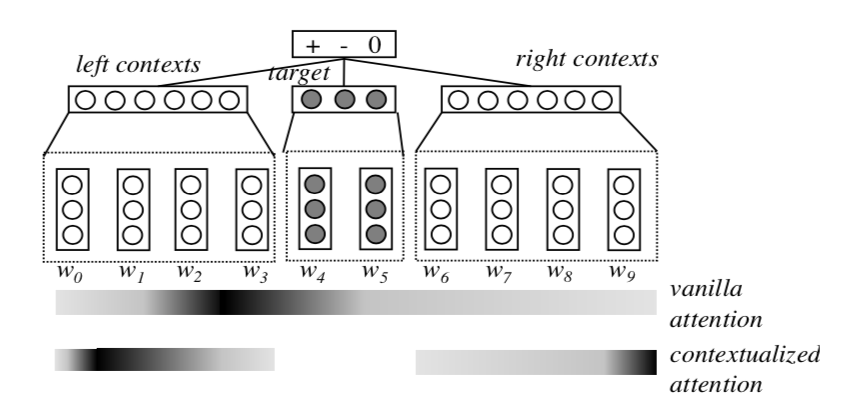
\includegraphics[width=0.8\linewidth]{bilstm-att-g.png}
    \caption{BILSTM-ATT-G模型结构}
    \label{fig:bilstm-att-g}
\end{figure}

在处理对某一目标的情感分析(Aspect-Term Sentiment Analysis or Target-oriented Sentiment Analysis)时,BILSTM-ATT-G(BiLSTM with Attentional Gates)~\cite{liu2017attention}除了考虑不同单词的重要性,还考虑了句子不同部分的重要性。图~\ref{fig:bilstm-att-g}显示了BILSTM-ATT-G的结构。它用目标将句子分成了左边、右边和目标三部分。首先,它使用与上面提到的简单attention模型来处理句子的左边部分、右边部分和目标;然后,利用attention模型的输出和最后一个隐层表示来计算一个门,并通过这个门对不同的部分的结果加权求和。这一方法对模型的效果有巨大的提升。从中可以看出,句子中不同的部分有着不同的重要性,gate方法可以很好地学习到这种重要性。

\subsection{GCAE}

\begin{figure}[ht]
    \centering 
    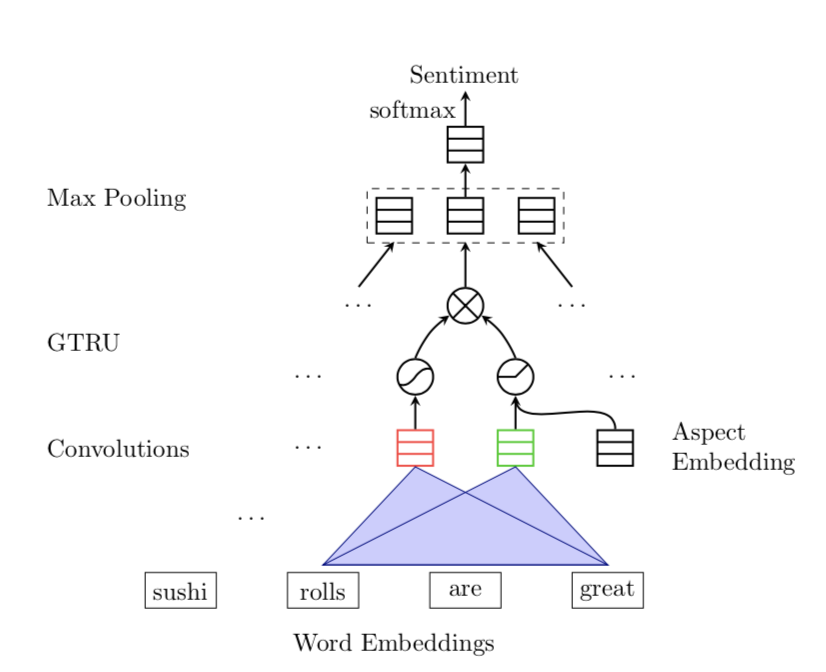
\includegraphics[width=0.8\linewidth]{gcae.png}
    \caption{GCAE模型结构}
    \label{fig:gcae}
\end{figure}

在前面所提到的模型中,LSTM等循环结构被用来处理单词的向量,得到句子的隐式表示。由于LSTM难以并行化,且当句子长度较长时训练困难,GCAE(Gated Convolutional Network with Aspect Embedding)开始尝试用CNN\cite{krizhevsky2012imagenet,grefenstette2014convolutional}解决处理句子。图~\ref{fig:gcae}显示了GCAE模型的结构。首先,GCAE用一维卷积处理句子输入,得到了句子的表示;然后对句子的单词和target的单词进行卷积,得到控制门;将二者相乘,得到了输入的表示。为了从不同粒度处理句子的特征,GCAE用到了多尺度的卷积,即使用了多个不同卷积核大小的卷积,并将它们的结果拼接起来。

\subsection{Memnet}

\begin{figure}[ht]
    \centering 
    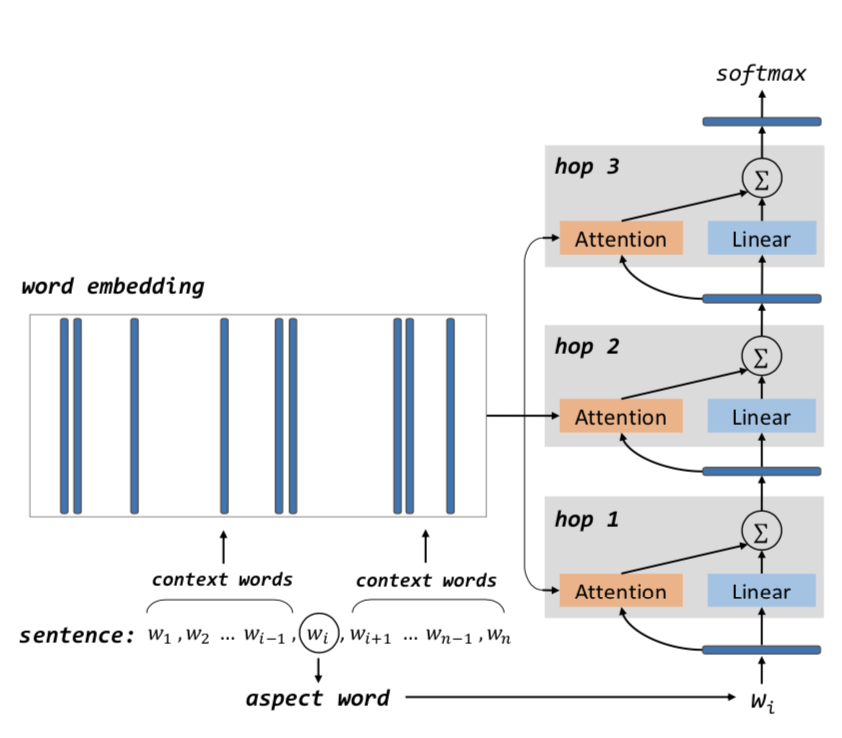
\includegraphics[width=0.7\linewidth]{memnet.png}
    \caption{Memnet模型结构}
    \label{fig:memnet}
\end{figure}

除了attention机制和gate方法,memory network~\cite{Weston2014Memory}也被应用到基于方面的情感分析中来。Memory network是一项机器学习技术,在问答系统中取得了优秀的表现~\cite{Weston2014Memory,Sukhbaatar2015End}。图~\ref{fig:memnet}显示了Memnet模型的结构。Memnet是一个多层结构。首先,它把单词的向量表示当作记忆单元,把目标单词的均值当作初始query;每层是一个attention的结构,上一层的结果作为下一层的query;各层结果之和作为最终的输出。Memnet利用了多层attention结构,它很好地解决了长期依赖的问题。但是,Memnet也存在一些问题:它直接使用单词的表示作为记忆单元,使得难以处理词组的信息;attention方法对单词的顺序不敏感,这样忽视了单词的时序信息。Memnet在处理需要推断、否定和比较的问题时遇到了困难。

\subsection{RAM}

\begin{figure}[ht]
    \centering 
    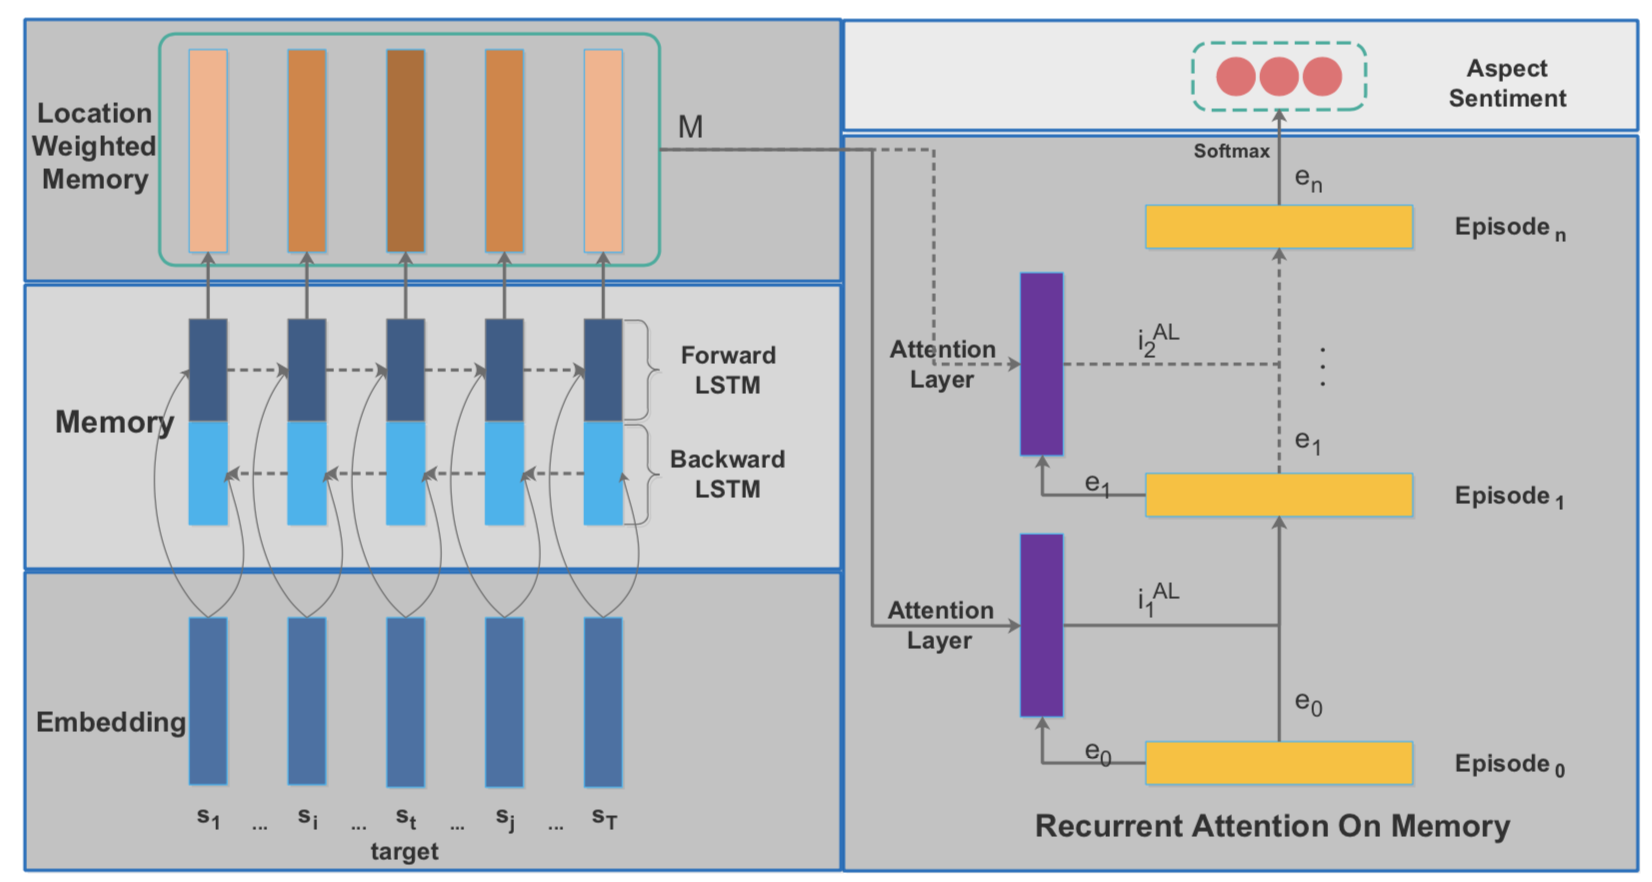
\includegraphics[width=0.7\linewidth]{ram.png}
    \caption{RAM模型结构}
    \label{fig:ram}
\end{figure}

针对Memnet的一些缺陷,RAM(Recurrent Attention Network)~\cite{Al2017Deep}。图~\ref{fig:ram}显示了RAM模型的结构。为了解决Memnet不善处理词组的问题,它使用双向LSTM来处理句子单词,得到了结合上下文的句子表示,并以此作为记忆单元;为了使模型具备一定的推断、否定和比较的能力,它不再简单地将上一层的输出作为下一层的query,而是利用一个\cite{cho2014learning}单元,得到下一层的query;同时,为了弥补Memnet不带有时序信息的问题,它引入了位置权重,使得与目标更近的单词权重更大。

\subsection{TNet}

\begin{figure}[h]
	\centering%
	\begin{subfigure}{0.5\textwidth}
		\centering
		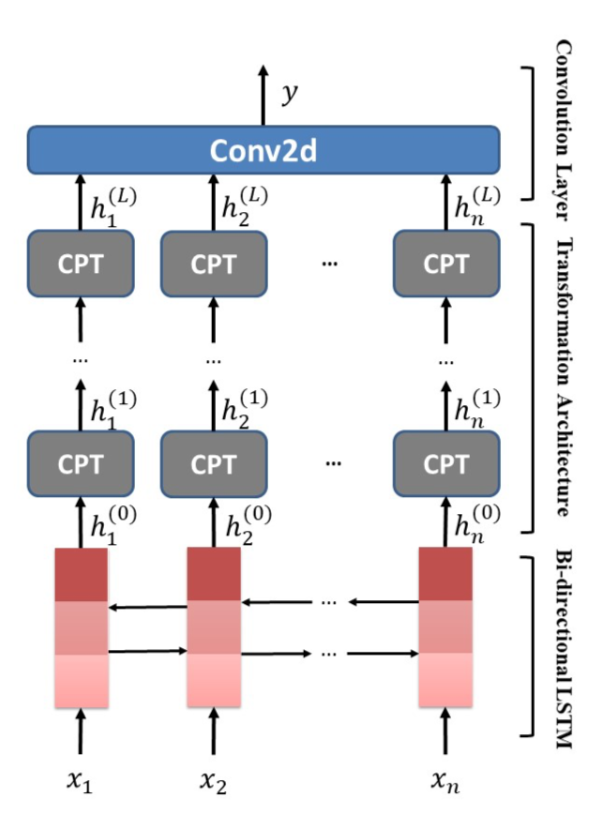
\includegraphics[width=0.5\textwidth]{tnet.png}
		\caption{整体结构}
	\end{subfigure}%
%	\hspace{4em}%
	\begin{subfigure}{0.5\textwidth}
		\centering
		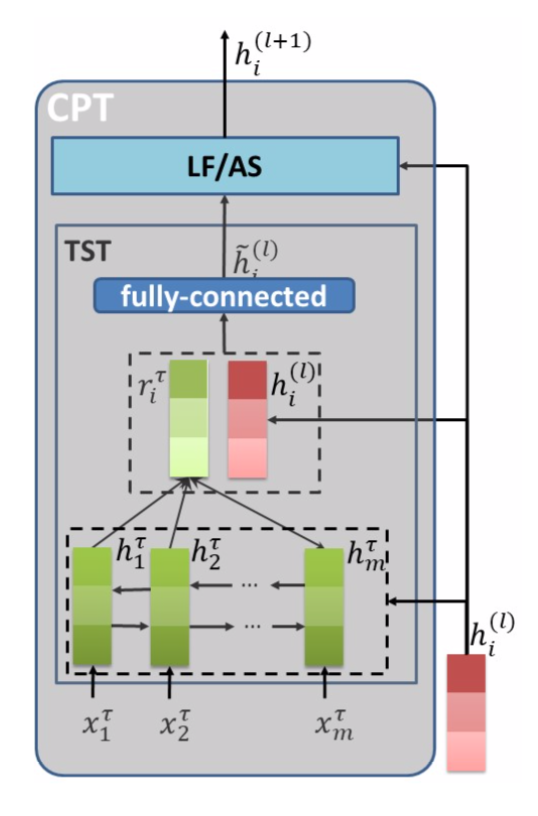
\includegraphics[width=0.5\textwidth]{cpt.png}
		\caption{CPT模块}
	\end{subfigure}
	\caption{TNet模型}
	\label{fig:tnet}
\end{figure}

TNet(Transformation Network)~\cite{Xin2018Transformation}集成了众多的技术,在多个公开数据集上取得了最佳的结果。图~\ref{fig:tnet}左图显示了TNet模型的结构。首先,它使用双向LSTM处理句子单词,得到结合上下文的表示,并以此作为记忆单元;然后,利用一个多层结构处理记忆单元;最后,利用二维卷积得到最终的句子表示。具体地,在每一层中,使用一个名为CPT(Context-Preserving Transformation)的结构,其结构如图~\ref{fig:tnet}右图所示。在CPT结构中,对每个句子中的单词,使用attention方法求得与句子单词相关的目标表示,将其与上一层的记忆单元通过一个单层映射得到下一层的记忆单元。同时,TNet还使用了更加复杂的位置权重。
\chapter{数据}
\label{cha:data}
在本章中,我们将介绍本文中使用的数据集,包括一些公开数据集如餐厅(Restaurant),笔记本电脑(Laptop),推特(Twitter)以及我们所构建的新闻驱动的股票预测数据集senti-stock。
\section{餐厅和笔记本电脑评论数据集}

\begin{table}[htb]
	\centering
	\begin{minipage}[t]{0.5\linewidth} % 如果想在表格中使用脚注,minipage是个不错的办法
		\caption[SemEval 2014 Task 4数据集统计信息]{SemEval 2014 Task 4数据集统计信息}
		\label{tab:stat}
		\begin{tabularx}{\linewidth}{Xlll}
			\toprule[1.5pt]
			{\heiti 数据集} & {\heiti 积极} & {\heiti 消极} & {\heiti 中性} \\\midrule[1pt]
			Laptop-Train &  994 & 870 & 464\\
			Laptop-Test & 341 & 128 & 169\\
			Restaurant-Train & 2164 & 807 & 637\\
			Restaurant-Test & 728 & 196 & 196\\
			\bottomrule[1.5pt]
		\end{tabularx}
	\end{minipage}
\end{table}

SemEval 2014 Task 4提供了一个基于方面的情感分析数据集,是在基于方面的情感分析领域应用最为广泛的数据集。基于方面的情感分析旨在提取句子中对某一方面或目标的情感极性。这一数据集由人工标注的餐厅Restaurant和笔记本电脑Laptop的评论组成。数据集分为训练集和测试集两部分。表\ref{tab:stat}显示了Restaurant和Laptop数据集的统计信息。从表中的数据可以看出,在训练集和测试集中,积极、消极、中性的标签分布并不均衡,尤其是笔记本电脑Laptop评论数据集。同时,训练数据的量并不是很大。这些特点给这一数据集增加了难度。Restaurant和Laptop数据集都是一个比较正式的数据,句子都比较完整,语法较规范。

我们在表\ref{tab:res-lap-case}中给出了餐厅和笔记本电脑评论的一些例子,目标由中括号圈出,正确的情感极性以下标的形式给出。可以看到,目标是句子中的一个子串,但其并不一定是一个单词,可能是一个短语;一个句子可能与多个目标有关,这些目标的情感极性可能不同。

\begin{table}[H]
	\centering
	\begin{minipage}[t]{0.8\linewidth} % 如果想在表格中使用脚注,minipage是个不错的办法
		\caption[Restaurant和Laptop数据集样本例子]{Restaurant和Laptop数据集样本例子}
		\label{tab:res-lap-case}
		\begin{tabularx}{\linewidth}{X}
			\toprule[1.5pt]
			{\heiti 样本示例} \\\midrule[1pt]
			The [food]\textsubscript{P} is uniformly exceptional, with a very capable [kitchen]\textsubscript{P} which will proudly whip up whatever you feel like eating, whether it's on the [menu]\textsubscript{O} or not. \\  \midrule[1pt]
			Our agreed favorite is the [orrechiete with sausage and chicken]\textsubscript{P} (usually the [waiters]\textsubscript{P} are kind enough to split the [dish]\textsubscript{O} in half so you get to sample both [meats]\textsubscript{O}).  \\ \midrule[1pt]
			One night I turned the freaking thing off after using it, the next day I turn it on, no [GUI]\textsubscript{N}, [screen]\textsubscript{N} all dark, [power light]\textsubscript{O} steady, [hard drive light]\textsubscript{N} steady and not flashing as it usually does. \\ 
			\bottomrule[1.5pt]
		\end{tabularx}
	\end{minipage}
\end{table}

\section{推特数据集}

\begin{table}[htb]
	\centering
	\begin{minipage}[t]{0.5\linewidth} % 如果想在表格中使用脚注,minipage是个不错的办法
		\caption[Twitter数据集统计信息]{Twitter数据集统计信息}
		\label{tab:twitterdataset}
		\begin{tabularx}{\linewidth}{Xlll}
			\toprule[1.5pt]
			{\heiti 数据集} & {\heiti 积极} & {\heiti 消极} & {\heiti 中性} \\\midrule[1pt]
			Twitter-Train & 1567 & 1563 & 3127 \\
			Twitter-Test & 174 & 174 & 346 \\
			\bottomrule[1.5pt]
		\end{tabularx}
	\end{minipage}
\end{table}

Twitter~\cite{dong2014adaptive}是一个由推特内容构成的数据集。这个数据集针对于对某一目标的情感分析问题,是由人工标注的。表~\ref{tab:twitterdataset}显示了该数据集的统计信息。推特Twitter数据集分为训练集和测试集两部分,从表\ref{tab:twitterdataset}中可以看出,推特Twitter数据集中训练集和测试集的标签分布相对来说还是比较均匀的。但推特数据集中的句子多比较口语化,涉及很多口语化的表达,句式不规范,甚至包含emoji表情等内容,这些都给这一数据集增加了难度。


\begin{table}[H]
	\centering
	\begin{minipage}[t]{0.8\linewidth} % 如果想在表格中使用脚注,minipage是个不错的办法
		\caption[Twitter数据集样本例子]{Twitter数据集样本例子}
		\label{tab:twitter-case}
		\begin{tabularx}{\linewidth}{X}
			\toprule[1.5pt]
			{\heiti 样本示例} \\\midrule[1pt]
				Awwwwww . The [Obama]\textsubscript{N} Family Vacation/Spring Break is cut short due to a few trivial matters concerning the future of our country. \\ \midrule[1pt]
				Damn you [Britney Spears]\textsubscript{N} for making such catchy songs ... \\ \midrule[1pt]
				Stranding at the checkout line ... Wow that picture of [Lindsay Lohan]\textsubscript{N} looks really bad . What happened to that poor girl ?! \\
			\bottomrule[1.5pt]
		\end{tabularx}
	\end{minipage}
\end{table}
%\begin{table}[H]
%	\centering  
%	\caption{Twitter数据集样本例子}
%	\label{tab:twitter-case}
%	\begin{tabular}{m{\textwidth}}
%		\hlinewd{1.2pt}
%		Awwwwww . The [Obama]\textsubscript{N} Family Vacation/Spring Break is cut short due to a few trivial matters concerning the future of our country. \\ \hline 
%		Damn you [Britney Spears]\textsubscript{N} for making such catchy songs ... \\ \hline 
%		Stranding at the checkout line ... Wow that picture of [Lindsay Lohan]\textsubscript{N} looks really bad . What happened to that poor girl ?! \\ \hlinewd{1.2pt}
%	\end{tabular}
%\end{table}

我们在表\ref{tab:twitter-case}中展示了一些推特数据集中的样例,其目标可能是一个单词或者是多个单词组成的短语;句子中包含大量的口语化表述,且句子并不一定严格符合语法规则。

\section{新闻驱动的股票预测数据集}

在之前的研究中用到的股票预测的数据集大都是不公开的。为此,我们构建了新闻驱动的股票预测数据集senti-stock并将其公开。本章将详细介绍我们如何收集数据、处理数据以及数据如何获取。图~\ref{fig:liuchengtu}显示了数据收集和处理的流程。

\begin{figure}[ht]
	\centering 
	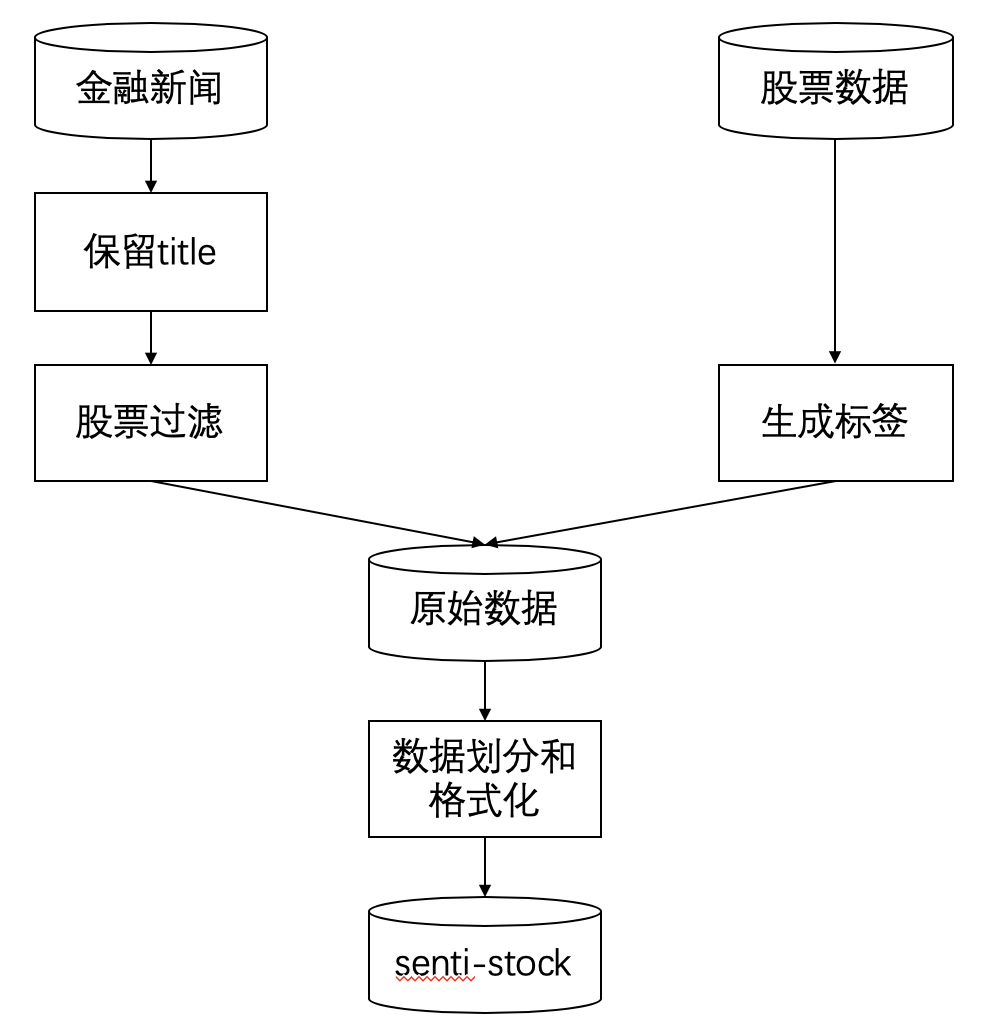
\includegraphics[width=0.5\linewidth]{LIUCHENGTU.png}
	\caption{senti-stock数据收集和处理流程图}
	\label{fig:liuchengtu}
\end{figure}

\subsection{收集数据}
我们选择美国股票市场作为研究对象。美国股市包含纽约证券交易所(New York Stock Exchange) 及纳斯达克证券市场 (Nasdaq Stock Market) 上市的股票 。道琼斯工业股票指数、纳斯达克指数和标准普尔500指数三大股指代表着美国股市的兴衰。美国股票市场于1811年建立,至今已经有两百年的历史。十八世纪,美国股票市场得到了初步发展;十八世纪末到十九世纪初,美国股市进一步发展,但市场操纵和内幕交易情况严重;十九世纪中期以前,美国股票市场进入规范化的发展时期;十九世纪中期至今,机构投资发展迅速,美国股票市场进入现代投资时代。因为其历史悠久,美国股票市场目前已经处于一个比较规范化的发展阶段。纽约证券交易所有超过三千支股票,包括一些历史悠久的大型企业,股份总值达到七兆亿美元;纳斯达克证券交易所是一个虚拟交易所,虽然历史较短,但有超过五千支股票,股票公司多为小型新公司。美国市场具有以下特点:
\begin{itemize}
	\item 规模大、市场成熟、运作规范、股价稳定;
	\item 证券市场管理严格、规范;
	\item 美国允许外国股份公司在美国证券市场发行股票并进行交易。
\end{itemize}

美国股票市场交易时间是周一到周五,美股没有单日股票涨跌幅限制,实行T+0交易制度,当天买入的股票可以当天卖出。
正因为美国股票市场具有上述特点,美国股票市场比中国股票市场更适合用来作为研究对象。

\begin{figure}[H]
	\centering 
	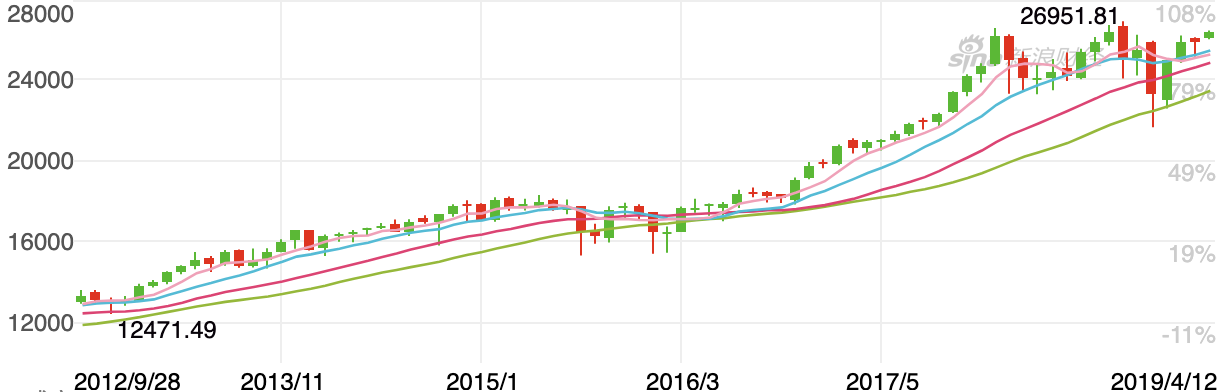
\includegraphics[width=0.8\linewidth]{djia.png}
	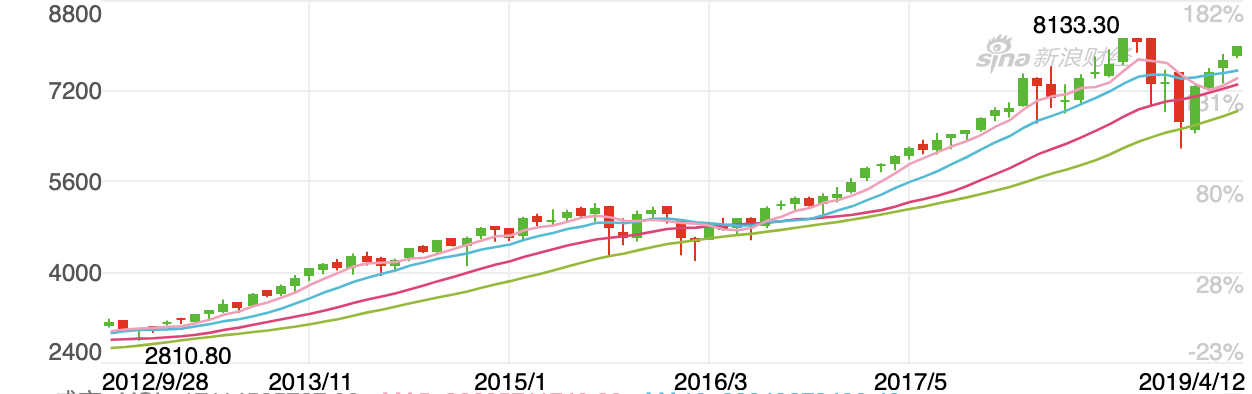
\includegraphics[width=0.8\linewidth]{nasdaq.png}
	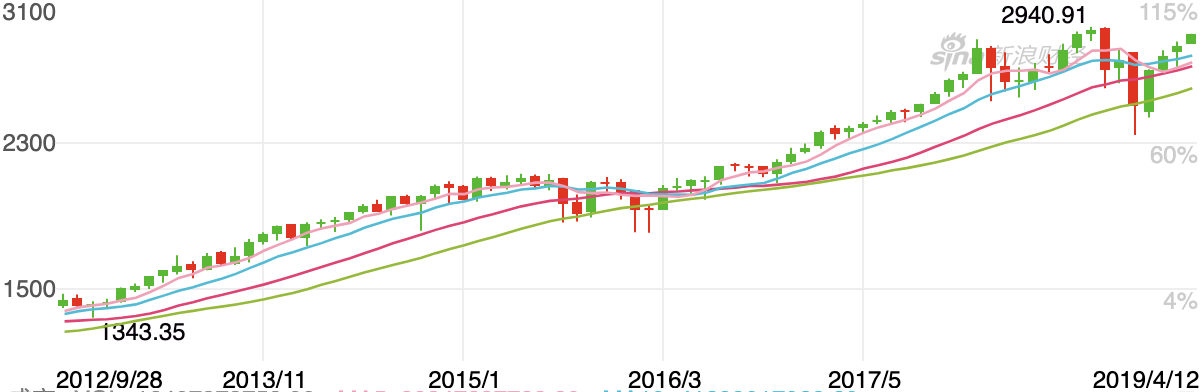
\includegraphics[width=0.8\linewidth]{sp500.png}
	\caption[美国市场三大指数]{美国市场三大指数:道琼指数、纳斯达克指数、标普500的月均线,图片来自新浪财经}
	\label{fig:index}
\end{figure}

\begin{table}[ht]
    \centering
    \begin{minipage}[t]{0.8\linewidth}
    	\caption[]{新闻样例}
    	\label{tab:newsexample}
    	\begin{tabularx}{1\linewidth}{lX}
    		\toprule
    		键 & 值 \\ \midrule
    		news\_type & topStory \\ 
    		symbol & AMD \\ 
    		name & Advanced Micro Devices Inc \\ 
    		date & 20161020 \\ 
    		title & AMD revenue beats on demand for chips used in gaming consoles \\ 
    		content & Chipmaker Advanced Micro Devices Inc reported a better-than-expected 23.2 percent increase in quarterly revenue helped by higher demand for graphics chips used in gaming consoles. \\ 
    		\bottomrule
    	\end{tabularx}
    \end{minipage}
\end{table}

我们主要从路透社收集新闻数据,从雅虎财经收集股票历史价格数据。

路透社(Reuters)是世界上最早创办的通讯社之一,也是目前英国最大的通讯社和西方四大通讯社之一。路透社是世界前三大的多媒体新闻通讯社,提供各类新闻和金融数据,在128个国家运行。路透社提供新闻报导给报刊、电视台等各式媒体,并向来以迅速、准确享誉国际。雅虎财经提供金融新闻、数据、评论等内容,包括股票历史数据、金融新闻报道和原创内容。雅虎财经提供的股票历史数据以准确及时而著称,并且雅虎财经提供了方便使用的数据接口。

为了从路透社网站和雅虎财经网站上抓取数据,我们使用了Scrapy框架。Scrapy\footnote{https://pypi.org/project/Scrapy/}是一个为了爬取网站数据,提取结构性数据而编写的应用框架。它可以应用在包括数据挖掘,信息处理或存储历史数据等一系列的程序中。其最初是为了 页面抓取 (更确切来说, 网络抓取)所设计的, 也可以应用在获取API所返回的数据(例如 Amazon Associates Web Services) 或者通用的网络爬虫。我们所使用的爬取数据的源码可以在github上获得\footnote{https://www.github.com/Cppowboy/stock\_data\_crawler}。

我们从路透社的网站上抓取了从2015年1月1日到2018年1月1日的美国市场的股票新闻数据。图~\ref{fig:index}显示了美国市场三大指数(道琼指数、纳斯达克指数、标普500指数)在近几年的变化波动趋势。可以看到,在2015年到2018年期间,美国股市整体上呈现稳定增长的趋势。我们得到了关于1297支股票的共计121096条新闻数据。这些新闻全部以JSON的格式保存。表~\ref{tab:newsexample}显示了我们一个新闻的样例。其中,news\_type指的是新闻的类型,包括"topStory"和"normal"两种。"symbol"是股票的代码。"name"是股票的全称。"date"是新闻的日期,格式为"\%Y\%m\%d"。"title"和"content"分别表示新闻的标题和内容。我们使用一个python包fix-yahoo-finance\footnote{https://pypi.org/project/fix-yahoo-finance/}来获取每支股票的历史价格数据。

%\begin{lstlisting}[language={Python}]
%	from pandas_datareader import data as pdr
%	import fix_yahoo_finance as yf
%	yf.pdr_override() 
%	
%	data = pdr.get_data_yahoo("SPY", start="2017-01-01", end="2017-04-30")
%	data = pdr.get_data_yahoo(["SPY", "IWM"], start="2017-01-01", end="2017-04-30")
%\end{lstlisting}

\begin{figure}[H]
	\centering 
	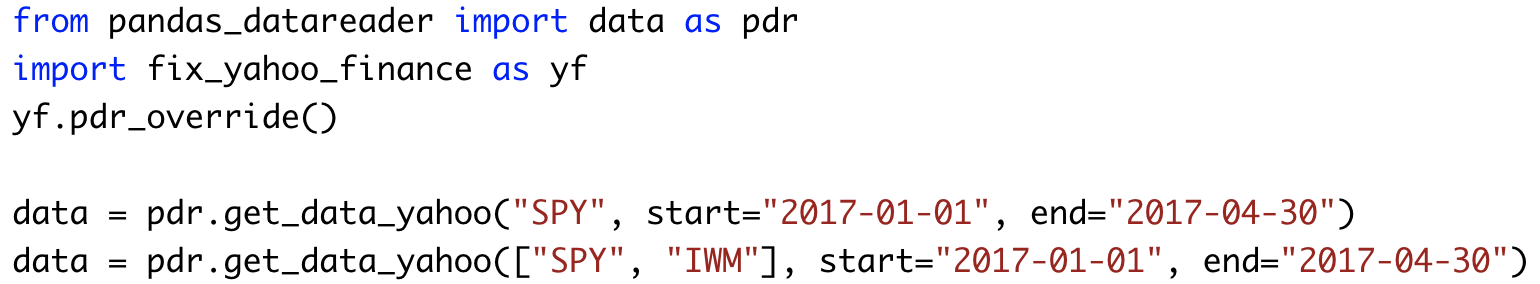
\includegraphics[width=0.8\linewidth]{sourcecode.png}
	\caption[]{fix-yahoo-finance代码示例}
	\label{fig:fix-yahoo-finance-source-code}
\end{figure}

图\ref{fig:fix-yahoo-finance-source-code}给出的fix-yahoo-finance的示例代码,我们利用这一工具得到了历史数据,即股票每天的收盘价。在这里,我们假设某支股票的涨跌仅与前一天、周、月的相关新闻有关,不受其他因素的影响。然后从短期(天)、中期(周)、长期(月)三个时间间隔去生成输出的标签~\cite{ding2014using}。三种不同的时间间隔的标签构成了Short、Middle、Long三个不同的数据集。如果股票收盘价格在下一天、周、月的涨幅超过1\%,则将标签设为$+1$;如果股票价格在下一天、周、月的跌幅超过1\%,则将标签设为$-1$;其他股票的标签设为$0$。

\subsection{处理数据}

之前的研究表明,新闻的标题更有助于预测新闻事件的影响,而新闻的内容往往包含太多不相关的信息。因此,我们只使用新闻的标题\cite{ding2014using}。
\begin{figure}[ht]
	\centering
	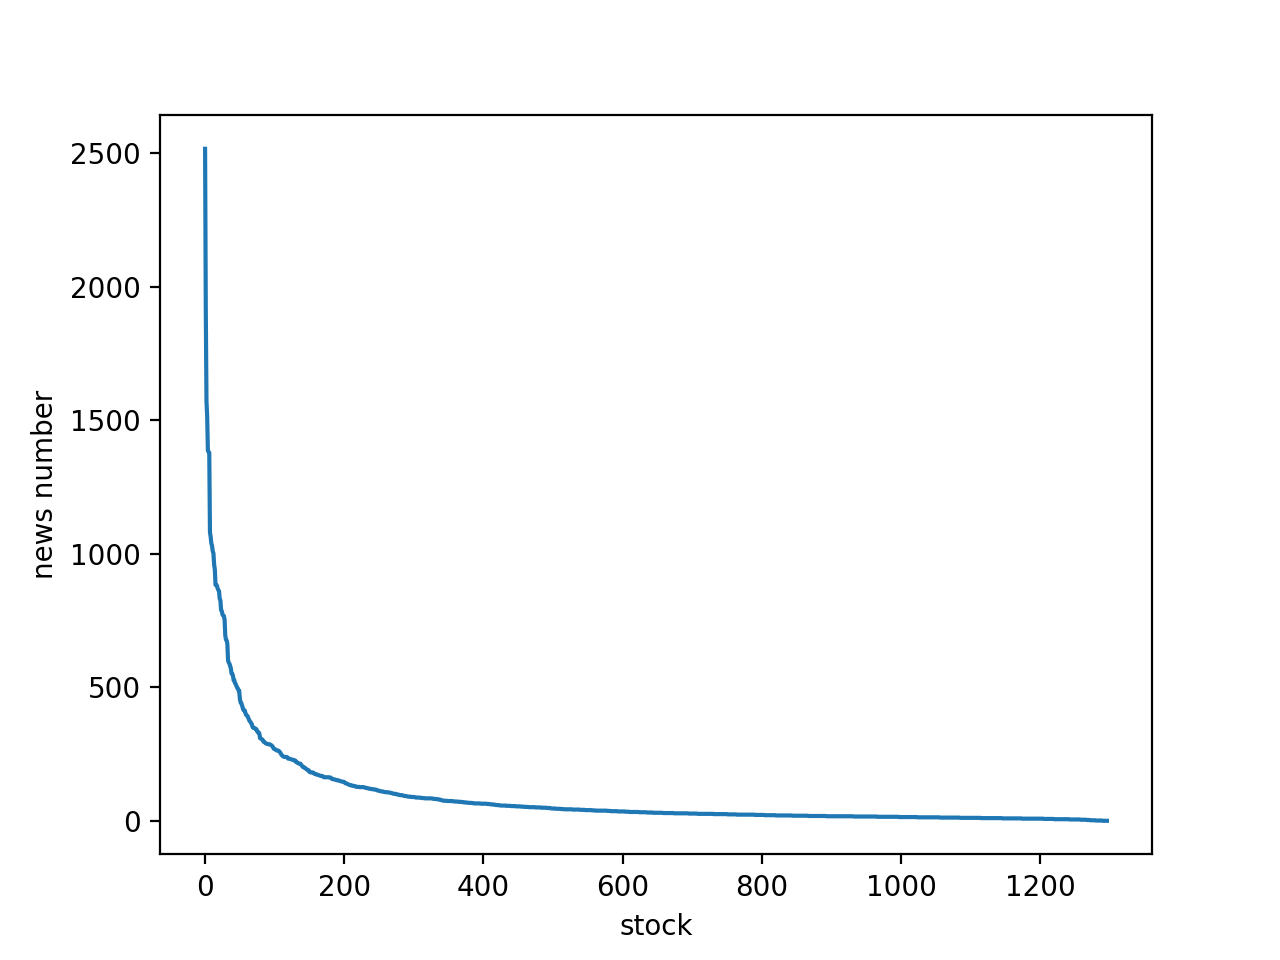
\includegraphics[width=0.8\linewidth]{all_stock_distribution.png}
	\caption{1297支股票的新闻数量分布}
	\label{fig:all-stock-distribution}
\end{figure}
图\ref{fig:all-stock-distribution}显示了全部股票的新闻数量分布。可以看到,大部分股票的相关新闻数量非常少,但有些比较知名的股票公司,其相关的新闻非常多。近期的研究\cite{ding2014using}显示,知名股票的预测准确率要高于不那么知名的股票,因为与知名股票相关的新闻事件数量更高。不知名股票的日常新闻非常少,以致于难以提取足够的信息来预测股票的变动。因此,我们对所有的股票进行简单的过滤,只保留新闻数量超过五百的股票,得到46支股票。这46支股票的新闻数量分布如图\ref{fig:good_stock_distribution}所示,这46支股票均是在美国市场中比较有知名度的股票。

\begin{figure}[ht]
	\centering 
	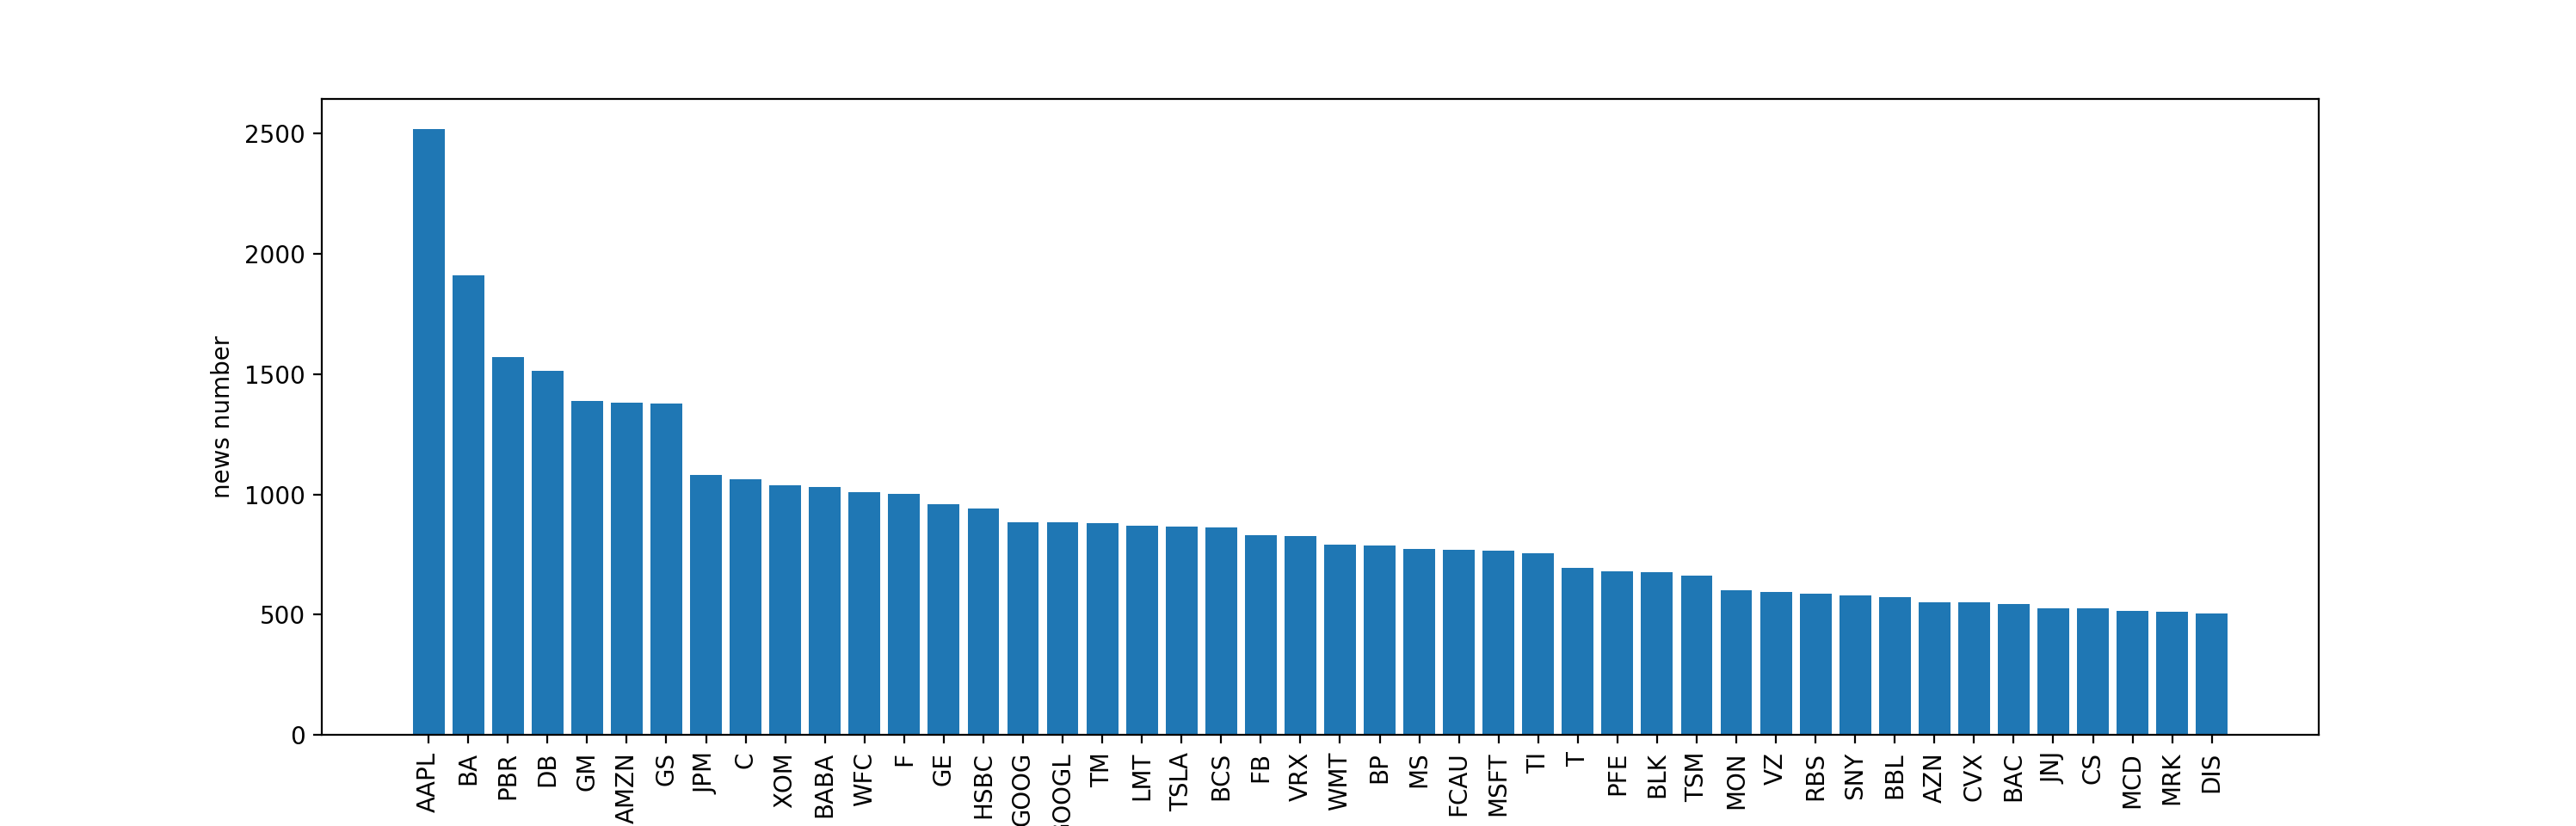
\includegraphics[width=\linewidth]{good_stock_distribution.png}
	\caption{新闻数超过五百的股票新闻数分布}
	\label{fig:good_stock_distribution}
\end{figure}

\begin{table}[ht]
	\centering 
	\begin{minipage}[t]{0.8\linewidth}
		\caption[]{数据集的统计信息}
		\label{tab:datasetstatistics}
		\begin{tabularx}{1\linewidth}{lXXX}
			\toprule
			数据集 & 全部数据 & 多标签数据 & 困难数据\\ \midrule
			Short-Train & 25496 & 3623 & 33 \\ 
            Short-Test & 6374 & 287 & 8 \\ 
            Middle-Train & 30637 & 4368 & 176 \\ 
            Middle-Test & 7660 & 353 & 17 \\ 
            Long-Train & 18324 & 2510 & 157 \\
			Long-Test & 4581 & 218 & 12 \\ 
			\bottomrule
		\end{tabularx}
	\end{minipage}
\end{table}

在完成上述处理后,我们将数据按照4:1的比例划分为训练集和测试集。表\ref{tab:datasetstatistics}显示了数据集的一些统计信息。其中,多标签数据指的是同一条新闻有多支相关的股票;困难数据指的是同一条新闻有多支相关股票且这些股票的涨跌情况不同,即同一条新闻对不同的股票有着不同的影响。困难数据是多标签数据的一个子集。

\begin{table}[ht]
	\centering
	\begin{minipage}[t]{0.8\linewidth}
		\caption{数据集中标签的分布}
		\label{tab:labeldistribution}
		\begin{tabularx}{\linewidth}{lXXX}
			\toprule 
			& $+1$ & $0$ & $-1$ \\ \midrule  
			Short-Train & 5483 & 141915 & 5098 \\ 
			Short-Test & 1388 & 3640 &1346 \\
			Middle-Train & 11716 & 8743 & 10178 \\
			Middle-Test & 2936 & 2207 & 2517 \\ 
			Long-Train & 9109 & 2470 & 6745 \\ 
			Long-Test & 2194 & 653 & 1734\\ 
			\bottomrule
		\end{tabularx}
	\end{minipage}
\end{table}

表\ref{tab:labeldistribution}显示了数据集中各类标签的分布情况。在短期标签的数据集中,大部分标签的类别都是$0$。这是因为在很短的时间(一天)内,股票的价格往往不会出现较大的变动。中期标签的数据集比另外两个数据集要更加均衡。长期数据集中,大部分标签的类别都是$+1$,这是因为在2015年到2018年之间,股市整体上呈现稳定上升的趋势。在这三种标签的数据集中,短期数据集和和长期数据集各类标签分布相对比较不均匀,因此相对容易,而中期数据集相对困难一些。

\subsection{公开数据}

我们的数据集senti-stock将会以xml的形式存储,其存储格式与SemEval 2014数据集格式一致\cite{pontiki2014semeval-2014},数据集可以从github上下载\footnote{https://www.github.com/Cppowboy/senti-stock}。

\begin{figure}[ht]
	\centering
	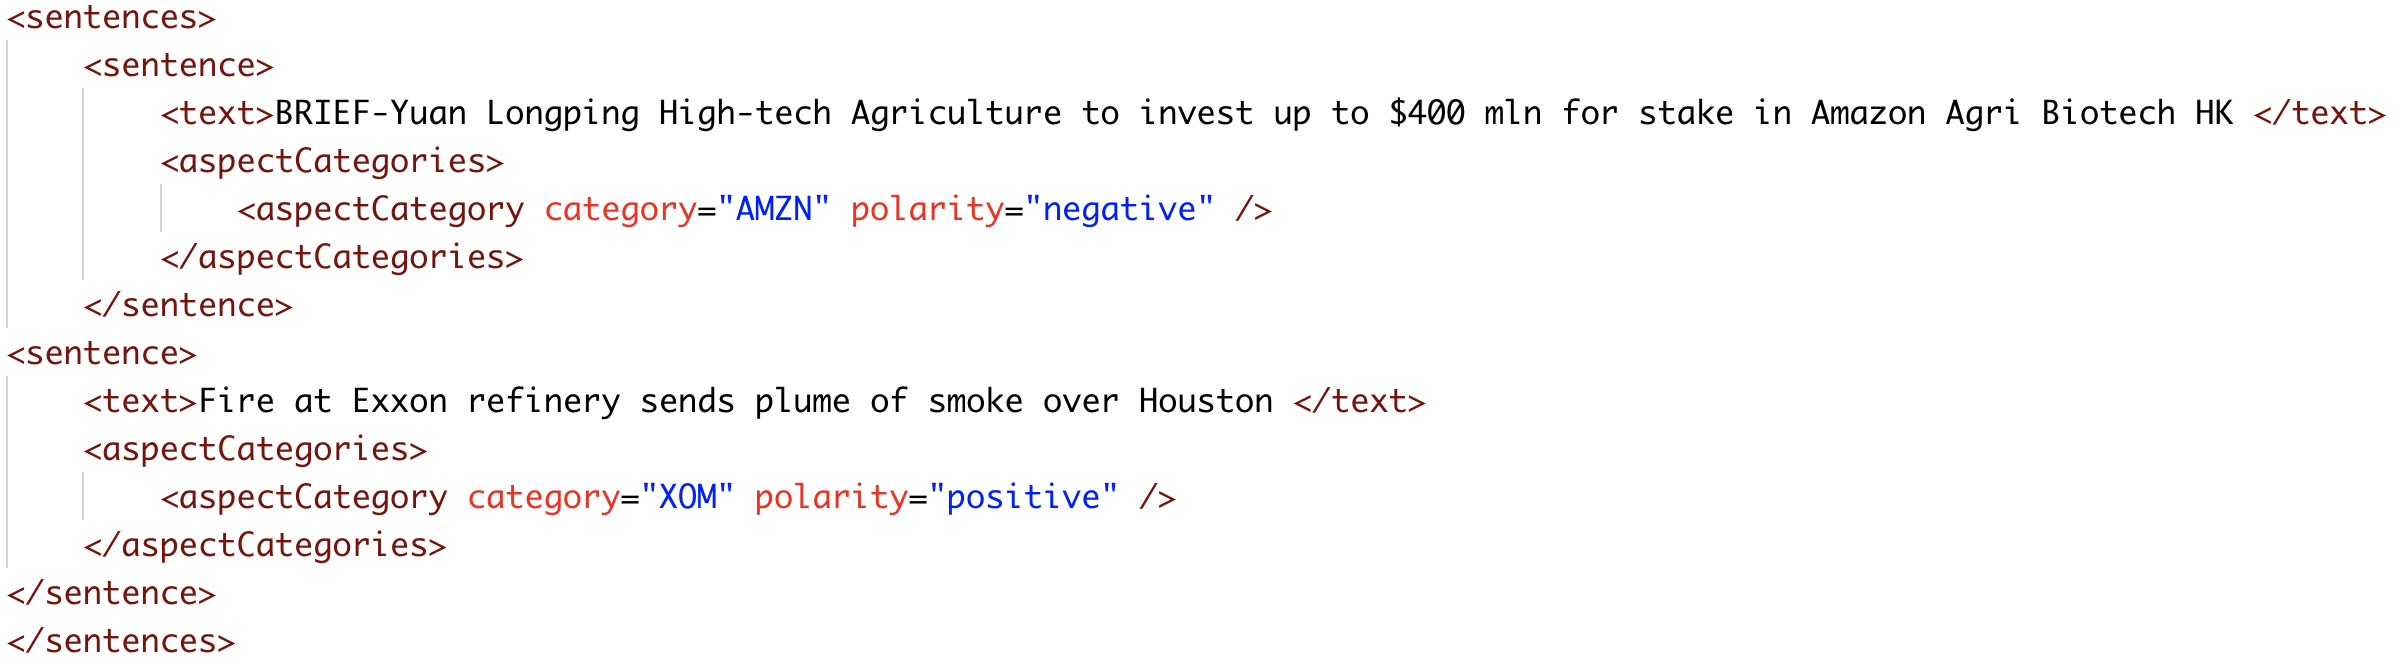
\includegraphics[width=\linewidth]{dataformat.png}
	\caption{senti-stock数据集格式}
	\label{fig:dataformat}
\end{figure}
图\ref{fig:dataformat}显示了senti-stock数据集的数据格式,text是新闻句子的内容,aspectCategory是各个与此新闻相关的股票,category属性是股票的代码,polarity属性是股票在下一个时间段内的涨跌情况。
\chapter{基于转换器和多尺度卷积的模型}
\label{cha:transformer}

为了更好地解决对某一目标的情感分析问题(Aspect-Term Sentiment Analysis, Target-oriented Sentiment Analysis),我们提出了使用转换器(Transformer)和多尺度卷积的模型。本章中,首先我们给出问题的形式化描述;然后,我们介绍转换器的结构;最后,介绍多尺度卷积的部分和目标函数。

\section{问题描述}

问题的输入是一个句子目标对$(w,w^\tau)$,其中目标$w^\tau=\{w^\tau_1,w\tau_2...w\tau_m\}$是句子$w=\{w_1,w_2...w_n\}$的子串,$m$是目标的长度,$n$是句子的长度。对某一目标的情感分析(Aspect-Term Sentiment Analysis, Target-oriented Sentiment Analysis)的目标是提取句子所表达的对目标的情感极性$y\in \{P, N, O\}$,$P$,$N$,$O$分别表示积极、消极和中立。比如,句子“great food but the service was dreadful!”对目标“food”的情感极性是积极的,对目标“service”的情感极性是消极的。

\section{模型介绍}

\begin{figure}[ht]
    \centering  
    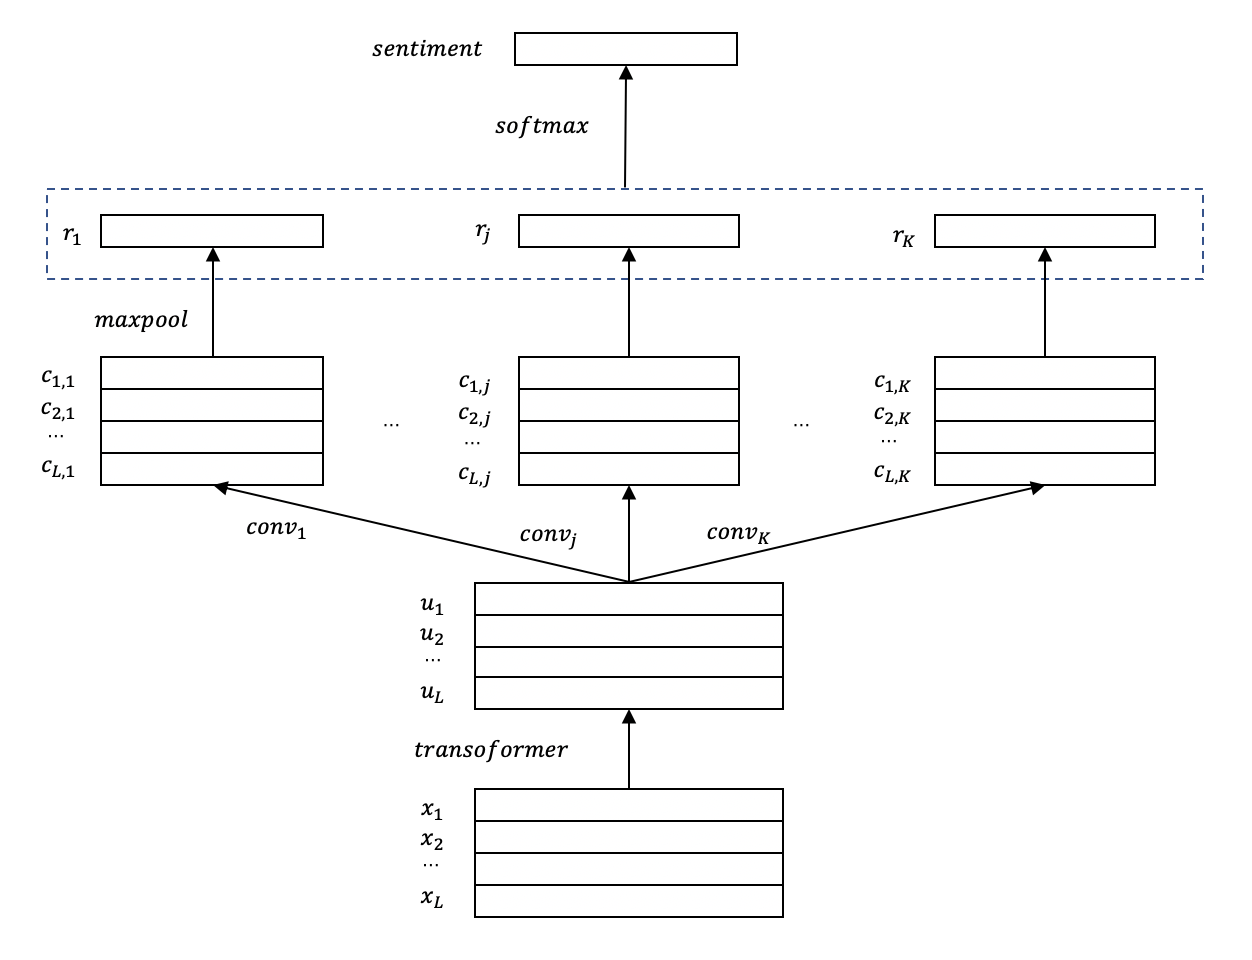
\includegraphics[width=0.8\linewidth]{transformer-model.jpg}
    \caption{基于transformer和多尺度卷积的模型}
    \label{fig:transformer-model}
\end{figure}

图~\ref{fig:transformer-model}显示了我们所提出的模型的主要结构。我们将目标和句子拼接起来,并用多层转换器结构来处理;多尺度卷积可以学习变长n-gram特征。

\section{转换器结构}

循环网络结构RNN和卷积神经网络CNN经常被用来将一个变长序列映射成一个固定长度的序列。循环网络结构RNN一般沿着序列的时间维度,逐个地生成隐层状态。循环网络RNN天然地具有时序性,这也使得循环网络结构在训练过程中难以被并行。当序列长度较长时,RNN往往难以训练。

卷积神经网络CNN通过局部感受野,获取输入序列的局部特征。但是,由于卷积的局部性,导致单层卷积难以学习长期的依赖关系;多层卷积可以弥补这一问题,但长期依赖的路径变长。

转换器(Transformer)\cite{NIPS2017_7181}不依赖循环网络结构和卷积神经网络,只通过自注意力机制就将输入序列映射到固定长度的输出序列。在本小节中,我们将简要地介绍转换器的结构。

\begin{figure}[ht]
    \centering 
    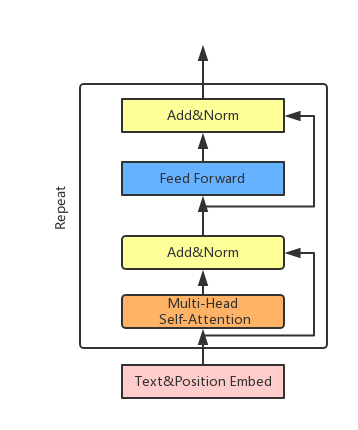
\includegraphics[width=0.5\linewidth]{transformer.jpg}
    \caption{Transformer结构}
    \label{fig:transformer}
\end{figure}

图~\ref{fig:transformer}显示了转换器(Transfomer)的结构。转换器(Transformer)是一个多层结构,每一层包括自注意力机制(self-attention)和前向网络。

\subsection{点积注意力机制}

点积注意力机制与常见的注意力机制不同,它的注意力权重是由点积求得的。对于query~$Q\in R^{T_q\times d_k}$,key $K\in R^{T_v\times d_k}$和value $V\in R^{T_v\times d_v}$,注意力机制的输出是
\begin{equation}
    Attention(Q,K,V)=softmax(\frac{QK^T}{\sqrt{d_k}})V
\end{equation}
其中,$T_q$是query的长度,$T_v$是key和value的长度,$d_k$是query和key的维度,$d_v$是value的维度。$\sqrt{d_k}$用来对权值进行缩放,保证了权值的稳定性。
\subsection{多头注意力机制}
转换器(Transformer)中并没有使用单一的注意力机制,而是用不同的线性映射将query,key,value映射$h$次。多次attention机制可以看作是单一注意力机制的一种嵌入模型。多个映射将query,key,value映射到了不同的子空间,多头注意力机制侧重于不同的值。
\begin{equation}
    \begin{aligned}
        MultiHead(Q,K,V)&=concat(head_1,head_2...head_h)W^O\\
        head_i&=Attention(QW^Q_i,KW^K_i,VW^V_i)
    \end{aligned}
\end{equation}
其中用到的映射都是不包含偏置的线性映射,其中$W^Q_i\in R^{d_{model}\times d_k}$,$W^K_i\in R^{d_{model}\times d_k}$,$W^V_i\in R^{d_{model}\times d_v}$是需要学习的参数,$d_{model}$是单词向量的维度。
自注意力机制(Self-Attention)是$Q$、$K$、$V$相同的多头注意力机制。
\begin{equation}
    SelfAttention(V)=MultiHead(V,V,V)
\end{equation}
\subsection{前向网络}
在转换器的每一层中,除了用到了注意力机制,还使用了一个两层全连接网络,使用relu激活函数。
\begin{equation}
    FFN(x)=relu(xW_1+b_1)W_2+b_2
\end{equation}
\subsection{词向量和柔性最大值传输函数}
与其他序列模型类似,我们将输入单词和输出单词映射为一个需要学习的向量,向量的维度是$d_{model}$。模型的最后,使用一个带有柔性最大值传输函数(softmax)激活函数的线性层得到预测结果。
\subsection{位置编码}
因为多头注意力机制和前向网络没有卷积层和循环结构,不能处理输入序列的时序信息,我们使用了位置编码来弥补这一缺点。这里用到的位置编码是在训练过程中学习得到的,而不是利用提前定义好的\cite{radford2018improving}。
\section{语言模型和预训练}

在本小节,我们对语言模型和使用转换器的语言模型做简要的介绍。一个统计语言模型通常构建为句子$w$的概率分布$P(w)$,这里$P(w)$实际上反映的是$w$作为一个句子出现的概率。对于一个由$n$个词按顺序构成的句子$w=\{w_1,w_2...w_n\}$,$P(w)$实际上求解的是字符串的联合概率,利用贝叶斯公式,链式分解如下:
\begin{equation}
    P(w)=P(w_1,w_2...w_n)=P(w_1)P(w_2|w_1)P(w_3|w_1,w_2)...P(w_n|w_1,w_2...w_{n-1})
\end{equation}
从上面可以看出,语言模型可以看成,在给定了前一个词的情况下,求下一个词出现的条件概率。在这里,我们使用的是基于转换器的语言模型。设$W_e$是词向量表示,$W_p$是位置编码,$h_l$表示第$l$层的中间结果。初始句子表示为
\begin{equation}
    h_0=UW_e+W_p
\end{equation}
我们用$transformer\_block$表示转换器的每一层。
\begin{equation}
    h_l=transformer\_block(h_{l-1})
\end{equation}
则最终的概率分布为
\begin{equation}
    P(w)=softmax(h_nW^T_e)
\end{equation}
语言模型的训练只需要句子本身,因此其训练数据非常的充足。之前的研究\cite{DBLP:conf/naacl/PetersNIGCLZ18,DBLP:journals/corr/abs-1810-04805,radford2018improving}表明,使用在大规模语料库上预训练的语言模型的参数,可以大大提升分类任务的效果。我们使用OpenAI GPT\cite{radford2018improving}提供的预训练的语言模型,将语言模型的输出用作特征。OpenAI GPT是在BooksCorpus数据集上训练的,它包括七千本书籍,内容包括了冒险、奇幻、史诗类作品。另一个数据集是1B
Word Benchmark\cite{Zhu2015Aligning},它与BookCorpus有类似的大小。在这个语料库上训练该语言模型,直到达到了18.4的困惑度(perplexity)。我们用预训练得到的参数去初始化转换器的参数,之后在对某一目标的情感分析任务中去调优这些参数。

本小节中使用的符号是为了解释语言模型的相关问题,与其他章节的符号无关,并不冲突。
\section{多尺度卷积}
我们把对某一目标的情感分析问题( Aspect-Term Sentiment Analysis, Target-oriented Sentiment Analysis)转化为一个序列对分类问题。具体地,我们把句子$w=\{w_1,w_2...w_n\}$和目标$w^\tau=\{w^\tau_1,w^\tau_2...w^\tau_m\}$拼接起来,在开头添加一个$start$记号,在结尾添加一个$end$记号,并在句子和目标之间添加一个$del$记号。拼接得到的序列记为$X$,$X=\{start,w_1,w_2...w_n,del,w^\tau_1,w^\tau_2...w^\tau_m,end\}=\{x_1,x_2...x_L\}$,其中$L=m+n+3$。将$X$输入到一个多层转换器结构当中,得到每个单词的表示。在这里,为了简洁,我们用下面的方式表示多层转换器结构。
\begin{equation}
    u_1,u_2...u_L=transformer(x_1,x_2...x_L)
\end{equation}
一般情况下,$start$记号的表示$u_1$被用来当作整个输入的表示。这种方式忽略了其它单词的表示,而这些信息可能会对预测正确的情感极性有着重要的作用。为了解决这一问题,我们使用多尺度的卷积来处理所有单词的表示。在句子中,有许多不同长度的短语。多尺度的卷积可以提取不同长度短语的特征。我们使用了多个不同卷积核大小的卷积层,并在序列的两端补零使不同卷积的输出大小保持一致。$K$是卷积的数量。
\begin{equation}
    c_{1,j},c_{1,j}...c_{L,j}=tanh(DepthwiseSeparableCNN_{j}(u_1,u_2...u_L))
\end{equation}
其中$j$表示的是第$j$个卷积,$j\in[1,K]$。这里,我们使用的是深度可分离卷积(Depthwise Separable Convolution)\cite{chollet2017xception,kaiser2017depthwise}。传统卷积网络中,利用一定大小的卷积核对特征进行局部的卷积,除此之外,在通道维度上,输入通道和输出通道上是全连接的。设输入通道数是$c_{in}$,输出通道数是$c_{out}$,则一维卷积的参数数量是$k\times c_{in}\times c_{out}$。而Depthwise Separable Convolution先使用$k$为卷积核的卷积,对每个输入通道的特征进行处理,再用卷积核为$1$的卷积对通道信息进行整合。Depthwise Separable Convolution的参数数量变为了$k\times c_{in}+c_{in}\times c_{out}$,参数数量大大地减少。

\begin{figure}[h]
	\centering%
	\begin{subfigure}{0.45\textwidth}
		\centering
		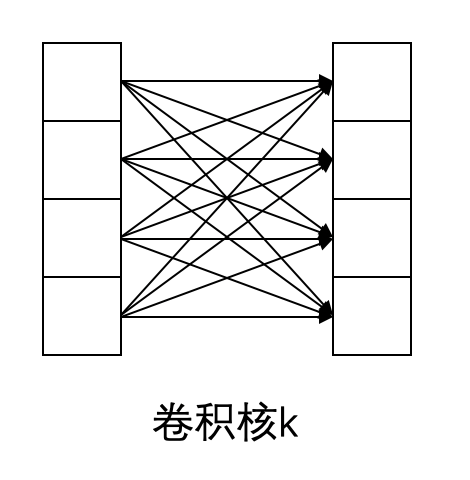
\includegraphics[width=0.45\textwidth]{normalcnn.png}
		\caption{传统CNN}
	\end{subfigure}%
	%	\hspace{4em}%
	\begin{subfigure}{0.55\textwidth}
		\centering
		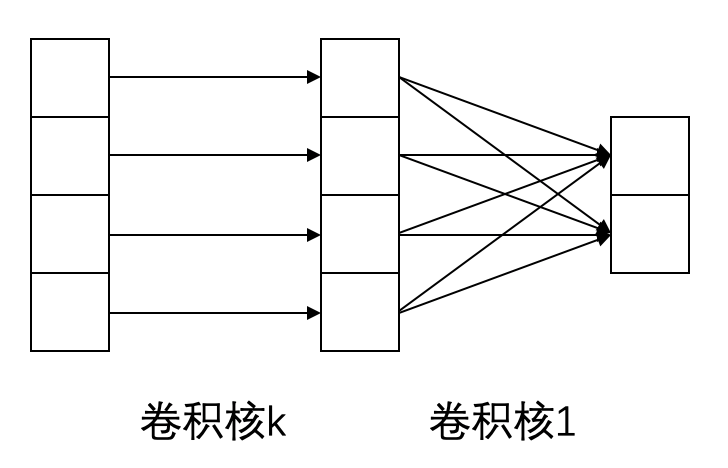
\includegraphics[width=0.55\textwidth]{depthwiseseparablecnn.png}
		\caption{Depthwise Separable CNN}
	\end{subfigure}
	\caption{两种卷积的对比}
	\label{fig:cnncompare}
\end{figure}
图\ref{fig:cnncompare}展示了普通卷积和Depthwise Separable Convolution和区别。与传统卷积相比,Depthwise Separable Convolution参数数量更少,具有更好的泛化性。
\begin{equation}
    r_j=max(c_{1,j},c_{2,j}...c_{L,j})
\end{equation}
把最大池化(max pooling)的输出结果沿最后一个维度拼接起来,得到句子的最终表示。
\begin{equation}
    r=concat([r_1,r_2...r_K],axis=-1)
\end{equation}
最后,使用带有softmax激活函数和全连接层得到预测结果。
\begin{equation}
    \hat{y}=softmax(Wr+b)
\end{equation}
其中$W$和$b$是全连接层的参数。
\section{目标函数}
训练过程中,我们的目标是最小化损失函数,损失函数是语言模型的损失函数和分类损失函数的和。
\begin{equation}
    Loss=Loss_{lm}+Loss_{clf}
\end{equation}   
语言模型的损失函数为
\begin{equation}
    Loss_{lm}=\sum_{i}\sum_{n}\hat{x_{i,n}}log(x_{i,n})
\end{equation}
其中,$x_i$是语言模型的第$i$个输出,$n$是单词的序号。分类损失函数是真实值$y$和预测值$\hat{y}$的交叉熵。
\begin{equation}
    Loss_{clf}=\sum_{i}\sum
    _{j}\hat{y_{i,j}}log(y_{i,j})
\end{equation}
其中,$i$是样本的序号,$j$是输出类别的序号。

\chapter{基于attention机制的多股票关系模型}
\label{cha: msra}
为了解决新闻驱动的股票预测问题,我们把它转化为针对某一方面的情感分析问题(Aspect-Category Sentiment Analysis)。我们提出了MSRA(Multi-Stock Relation using Attention mechanism,使用attention的多股票关系模型)模型,该模型包括情感分析模块和股票关系模块。在本章中,我们首先给出总是的形式化描述,并简要介绍模型的结构,然后分别介绍情感分析模块和股票关系模块。
\begin{figure}[H] % use float package if you want it here
    \centering
    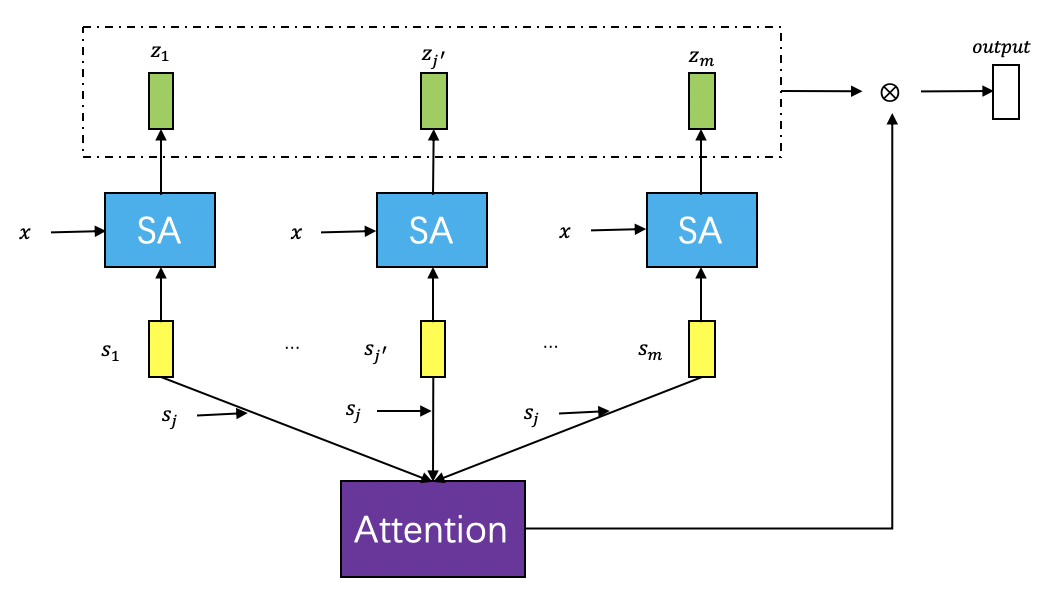
\includegraphics[width =\linewidth]{figures/stock-relation.png}
    \caption{MSRA模型结构}
    \label{fig: modelstructure}
\end{figure}

\section{问题描述}

问题的输入包括一支股票$s$以及一条与这支股票相关的新闻$w =\{w_1, w_2...w_n\}$,其中$n$是新闻句子的长度。句子相应的词向量表示是$x =\{x_1, x_2...x_n\}$。我们使用股票向量$s_j$来表示第$j$支股票,其中$j = 1, 2...m$,$m$是所有股票的数量。问题的输出是股票价格在下一个时间段内将会如何变化$y\in \{+1, 0, -1\}$,其中,$+ 1$表示股票的价格将会在下一天、周、月之后上涨,$- 1$表示股票的价格将会在下一天、周、月之后下跌,其它的为$0$。$C = 3$是输出标签的数量。比如,“微软收购诺基亚的手机部门”将会使微软(MSFT)的股票价格上涨,诺基亚(NOK)的股票价格下跌。
\section{模型结构}
图~\ref{fig: modelstructure}展示了模型的基本结构。我们使用情感分析模块提取与股票$j$相关的新闻$w$的情感表示;使用点积attention来学习股票之间的相关关系。所有股票的情感表示的加权和被用来作为输入的最终表示。最后使用带有softmax激活函数的全连接得到输出结果。
\section{股票向量}
在预测股票价格变化时,股票相关的信息有着重要的作用。同一条新闻,对不同的股票可能会产生完全不同的影响。为了更好地利用股票相关的信息,我们提出了股票向量的概念。我们为全部的股票构建一个词表,并为每支股票创建一个向量表示。向量$s_i\in R ^ {d_s}$表示的是第$i$支股票的向量表示,其中$d_s$表示的是股票向量的维度。$S\in R ^ {d_s\times | S |}$由全部的股票向量组成。据我们所知,这是第一次提出股票向量的概念。
\section{情感分析模块}

\begin{figure}[ht]
    \centering
    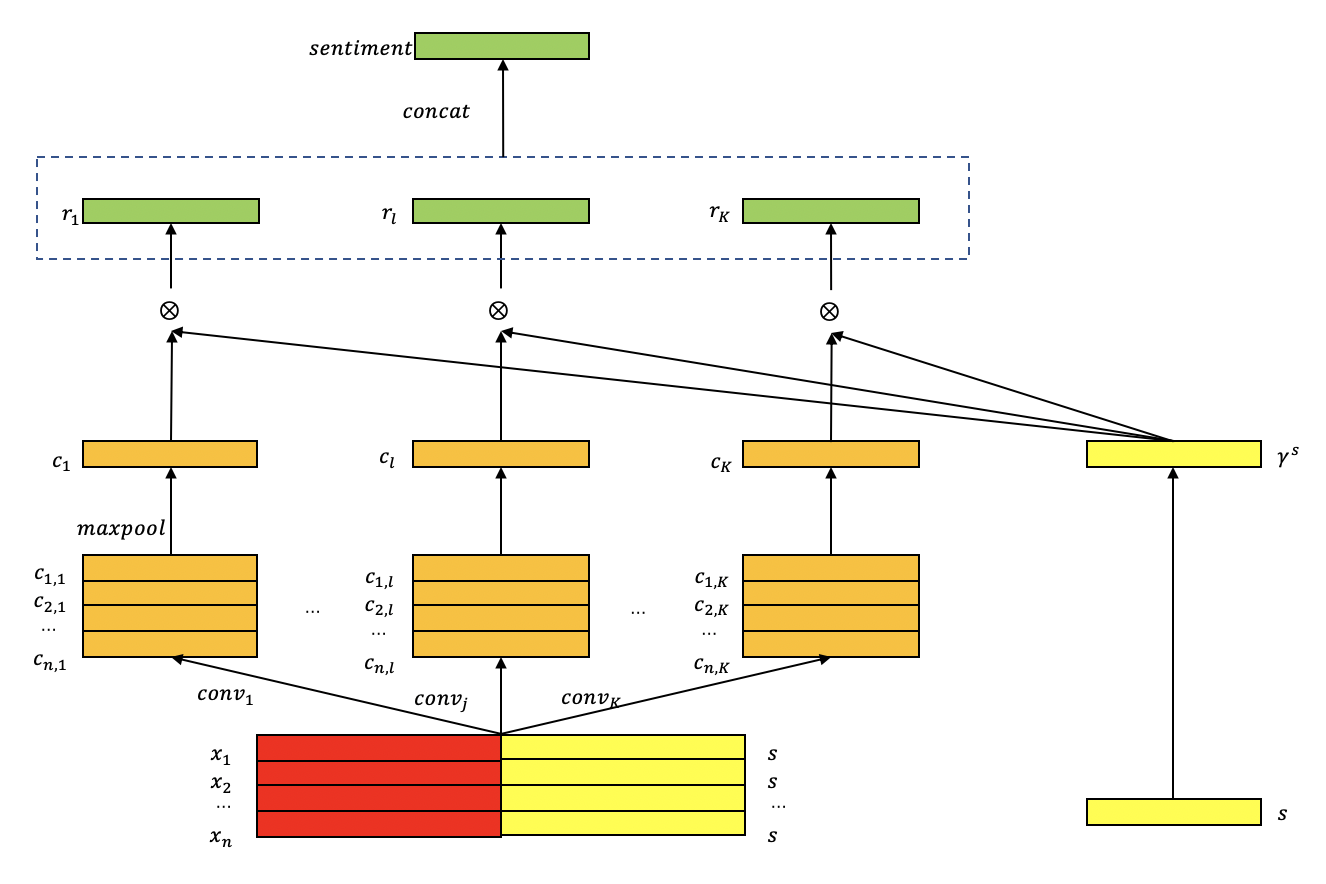
\includegraphics[width= 0.8\linewidth]{sentiment-analysis.png}
    \caption{情感分析模块}
    \label{fig: sentiment}
\end{figure}

如图~\ref{fig: sentiment}所示,情感分析模块使用了带有股票系数的多尺度卷积。

\subsection{多尺度卷积}
我们利用多尺度卷积来处理词向量。自然语言处理中常使用LSTM来处理句子序列,LSTM沿着时间维度,逐次计算下一个时间的隐层状态,从而将变长的序列转化为了定长输出。然后,因为LSTM的时序性,使得它难以并行化。CNN最初用于图片分类,CNN通过局部感受野,能够提取局部的特征。多层CNN在图像相关领域取得了非常优秀的表现,然而,CNN在自然语言处理领域一直没有得到很好的应用。直到TextCNN\cite{kim2014convolutional}提出,CNN才开始在自然语言处理中有所表现。相比于LSTM,CNN使用卷积核处理序列中局部的序列,更易于并行化。为了更好地结合股票相关信息,我们将句子的词向量$x_i$与股票向量$s$拼接起来。
\begin{equation}
    u_i = concat(x_i, s)
\end{equation}
卷积操作结合相邻的若干个单词的信息,相当于不同长度短语的特征。多尺度卷积使用了多个不同卷积核大小的卷积层,这样,可以提取不同长度的短语的特征。
\begin{equation}
    c_{i, l} = relu(u_{i: i+k_l}*W_l+b_l)
\end{equation}
其中,$W_l$和$b_l$是第$l$个卷积的参数,$k_l$是第$l$个卷积的卷积核大小, $l = 1, 2...K$,$K$是不同尺度卷积的数量。$relu$激活函数的定义如下。
\begin{equation}
    relu(x) =\begin{cases}
        x & x > 0 \\
        0 & x\le 0
    \end{cases}
\end{equation}
Max-pooling层选取值最高的特征,其思想在于把最重要的特征选取出来。同时,max-pooling层可以将变长的序列转化为固定的长度,方便后续的处理。
\begin{equation}
    c_l = max(c_{1, l}, c_{2, l}...c{n, l})
\end{equation}
之前的研究表明\cite{kim2014convolutional},多层CNN在自然语言处理中表现并不突出,却使得模型更深,更加难以训练,因此,我们这里只使用了单层卷积,并未使用多层的CNN结构。
\subsection{股票系数}
不同的股票具有不同的特性,有些股票更倾向于上涨,有些股票更倾向于下跌。为了更好地利用股票的特性,我们计算股票系数,它反映了股票的信息。
\begin{equation}
    \gamma ^ s = tanh(W_sx ^ s+b_s)
\end{equation}
其中, $W_s$和$b_s$是需要学习的参数。$tanh$函数的定义如下:
\begin{equation}
    tanh(x) =\frac{e ^ x-e ^ {-x}}{e ^ x+e ^ {-x}}
\end{equation}
我们用按元素的乘法将股票系数和句子表示结合起来。这里使用按元素的乘法,股票系数起到了对原有特征进行缩放的作用,从而使得本来的特征带有了股票的相关信息。
\begin{equation}
    r_l = c_l\otimes \gamma ^ s
\end{equation}
全部卷积的结果拼接起来,得到句子的最终表示。
\begin{equation}
    r = concat(r_1, r_2...r_K)
\end{equation}
\section{股票关系模块}
股票公司之间的竞争、合作、上游、下游关系,可能会影响股票价格的变动。比如,“亚马逊向中国及其他七个国家的卖家提供贷款”对亚马逊(AMZN)来说是一条积极的新闻,它将会使得亚马逊的股票价格上升;同时,它也会对亚马逊在中国的竞争者阿里巴巴(BABA)造成消极的影响,使得其股票价格下跌。我们使用点积attention来学习股票之间的相互关系。为了简便,我们使用下面的公式来表示情感分析模块的输出。
\begin{equation}
    z_{j'}=SA(x,s_{j'})
\end{equation}
其中,$j'=1, 2...m$是股票的序号。Attention的权重通过下面的公式求得。我们把所有股票的情感表示的加权和作为输入的最终表示。
\begin{equation}
    \begin{aligned}
        \alpha_{j'}&=\frac{s^T_{j}s_{j'}}{\sum_{j'=1}^{m}s^T_{j}s_{j'}}
        z &= \sum_{j'=1}^{m} \alpha_{j'}z_{j'}
    \end{aligned}
\end{equation}
\section{目标函数}

最后,由全连接层和softmax激活函数得到最终的预测结果。

\begin{equation}
    \hat{y}=softmax(Wz+b)
\end{equation}
其中,$W$和$b$是需要学习的参数。目标函数是实际值$y$和预测值$\hat{y}$之间的交叉熵。
\begin{equation}
    loss=\sum_{p} ^ {N}\sum_{c} ^ {C}\hat{y_{i, j}}log(y_{i, j})
\end{equation}
其中,$p$是样本序号,$c$是类别序号,$N$是样本数量,$C$是类别数量。

\chapter{实验}
\label{cha:experiment}
在本章中,我们分别介绍对某一目标的情感分析(Aspect-Term Sentiment Analysis or Target-oriented Sentiment Analysis)和新闻驱动的股票预测的实验设置及实验结果。

\section{对某一目标的情感分析}
在本小节,我们介绍对某一目标的情感分析(Aspect-Term Sentiment Analysis or Target-oriented Sentiment Analysis)的实验。这里,我们使用的是基于transformer和多尺度卷积的模型。
\subsection{实验设置}
我们在餐厅(Restaurant)、笔记本电脑(Laptop)、推特(Twitter)三个公开数据集上进行了实验。这三个数据集均在第~\ref{cha:data}章中有所介绍。我们沿用了之前工作中数据预处理的方法~\cite{Xin2018Transformation,Tang2015Effective},我们除去了一些冲突的标签,所有单词均转化为小写,不去除任何的停止词、符号、数字。我们使用nltk\footnote{http://www.nltk.org/}工具提供的分词工具对全部的句子进行分词。所有的句子都使用“PAD”字符补齐成最大长度。

我们使用准确率和macro-averaged F1 score作为评价指标。对每一类来说,精确率$P=\frac{TP}{TP+FN}$,召回率$R=\frac{TP}{TP+FP}$,F1 score由$\frac{2PR}{P+R}$求得。Macro-averaged F1 score是所有类别的F1 score的均值~\cite{Tang2015Effective}。

我们与下列模型进行了对比:
\begin{itemize}
    \item Majority把训练集中出现频率最高的类别作为预测类别;
    \item SVM是支持向量机模型,它使用的是人为构建的n-gram特征、解析特征和语义特征~\cite{kiritchenko2014nrc-canada-2014};
    \item AE-LSTM是一个将目标和句子拼接起来作为输入的LSTM模型;
    \item ATAE-LSTM对AE-LSTM进行了扩展,利用attention机制选取最重要的单词~\cite{wang2016attention-based};
    \item IAN利用交互式地方式,分别使用attention方法计算句子和目标的表示~\cite{ma2017interactive};
    \item BILSTM-ATT-G使用控制门来控制目标左边、右边部分的重要性~\cite{liu2017attention};
    \item GCAE使用卷积神经网络和控制门,得到了更高的准确率,更容易并行化~\cite{xue2018aspect};
    \item {Memnet}将词向量当作记忆单元,使用多层attention方法来得到最终表示,为克服attention机制不能获取时序信息的缺点,它还使用了位置权重~\cite{tang2016aspect};
    \item RAM对Memnet做出了改进,它使用双向LSTM的结果作为记忆单元,使用GRU来生成下一层的表示,同时使用了与Memnet不同的位置权重~\cite{Al2017Deep};
    \item TNet提出生成与目标相关的句子表示,同时结合上下文信息。\cite{Xin2018Transformation}.
\end{itemize}
我们使用pytorch\footnote{https://pytorch.org}框架实现了这些模型中除IAN之外的模型,并使它们的实验结果尽可能地与原论文相似。每个模型都是独立训练的。我们使用的是GloVe~\cite{pennington2014glove}词向量来初始化我们的词向量,并在训练的过程中调整词向量的值。句子的最大长度设为30。
在我们的模型中,我们使用的模型参数设置与OpenAI GPT~\cite{radford2018improving}一致。具体地,transformer的层数是12,多头attention的head数是12,词向量的维度设为768,中间层的维度设为了3072。我们首先加载OpenAI GPT~\cite{radford2018improving}的预训练参数,然后与后续结构一起进行调优。我们使用了五个不同的卷积核,卷积核大小从1到5。卷积的输出通道数设为100。我们使用Adam~\cite{kingma2014adam}优化器,学习率设为6.25e-5。模型在20轮训练内就得到了最好的效果。
\subsection{实验结果}

\begin{table}[ht]
    \centering
    \caption[对某一目标的情感分析实验结果]{对某一目标的情感分析实验结果(\%),带“*”的实验结果是从原文中获取的}
    \label{tab:result}
    \begin{tabular}{lcccccc}
    \hlinewd{1.5pt}
    \multirow{2}{*}{Models} & \multicolumn{2}{l}{Restaurant} & \multicolumn{2}{l}{Laptop} & \multicolumn{2}{l}{Twitter} \\ \cline{2-7} 
                            & ACC       & Macro-F1      & ACC     & Macro-F1    & ACC     & Macro-F1     \\ \hline
    Majority                &65.00           &-              &53.45         &-            &50.00         &22.22         \\
    SVM                     &80.89           &-              &72.10         &-            &63.40         &63.30         \\ 
    LSTM                    &76.70           &63.57          &69.28         &63.30        &66.04         &63.46         \\
    ATAE-LSTM               &77.23           &63.73          &69.44         &63.46        &71.24         &69.19         \\
    IAN                     &78.60$^*$       &-              &72.10$^*$     &-            &-             &-             \\
    BILSTM-ATT-G            &79.20           &67.07          &71.32         &64.88        &71.68         &70.37         \\
    GCAE                    &78.12           &62.50          &70.38         &64.02        &72.40         &70.89         \\
    MemNet                  &77.86           &64.47          &68.18         &62.46        &69.80         &66.86         \\
    RAM                     &78.30           &65.42          &71.63         &66.73        &71.24         &68.75         \\
    TNet                    &78.39           &65.37          &73.98         &68.64        &72.11         &70.01         \\ \hline
    Ours                    &84.91           &76.40          &78.37         &74.05        &74.86         &73.63         \\ \hlinewd{1.5pt}
    \end{tabular}
    \end{table}
表~\ref{tab:result}显示了对某一目标的情感分析的实验结果。我们的模型在Restaurant、Laptop、Twitter数据集上均取得了最佳的实验结果。我们在Restaurant数据集上取得了84.91\%的准确率(提升6.52\%),在Laptop数据集上取得了78.37\%的准确率(提升4.39\%),在推特数据集上取得了74.86\%的准确率(提升2.75\%)。

在所有的神经网络模型中,LSTM模型效果最差。ATAE-LSTM考虑到了目标并使用了attention方法,效果有所提升。IAN使用了句子对目标的attention和目标对句子的attention,更进一步提升了实验效果。BILSTM-ATT-G和RAM在Restaurant和Laptop上的实验效果较好,但在Twitter数据集上效果提升并没有那么大,可见LSTM不擅长处理Twitter数据中大量的口语化文本。TNet使用了CNN和LSTM,并在三个数据集上都取得了不错的效果。

不同于这些模型,我们的模型使用transformer提取句子特征,更易于处理长期依赖关系,易于并行。我们的模型利用多尺度卷积,从不同粒度提取特征。我们的模型在三个数据集上的实验效果比其他几个模型要好。
\subsection{预训练}
为了证明transformer预训练的效果,我们进行了对比实验:一组使用预训练的transformer参数,另一组完全随机初始化参数,并从头开始进行训练。
\begin{table}[h]
    \centering
    \caption{预训练的作用}
    \label{tab:pretrain}
    \begin{tabular}{lcccc}
         \hlinewd{1.5pt}
     \multirow{2}{*}{\textbf{Models}} & \multicolumn{2}{c}{Restaurant} & \multicolumn{2}{c}{Laptop} \\
     \cline{2-5}
                                      & ACC & Marco-F1 & ACC & Marco-F1 \\
    \hline
         w/o pre-training & $69.20$ & $48.16$ & $64.89$ & $59.25$ \\
         w/ pre-training & $84.91$ & $76.40$ & $78.37$ & $74.05$ \\
    \hlinewd{1.5pt}
    \end{tabular}
\end{table}
表~\ref{tab:pretrain}显示了对比实验的实验结果。当不使用预训练的参数时,实验效果大大下降。在预训练的过程中,深层transformer模型通过前几个单词去预测下一个单词;在这一过程中,模型学习到了语言的表示方式,并将这些知识迁移到后续的任务当中。

\subsection{多尺度卷积}
为证明多尺度卷积的重要性,我们将模型中的多尺度卷积去掉,对比了简化后的模型与完整模型的实验效果。
\begin{table}[h]
    \centering
    \caption{多尺度卷积的作用}
    \label{tab:cnn}
    \begin{tabular}{lcccc}
         \hlinewd{1.5pt}
     \multirow{2}{*}{\textbf{Models}} & \multicolumn{2}{c}{Restaurant} & \multicolumn{2}{c}{Laptop} \\
     \cline{2-5}
                                      & ACC & Marco-F1 & ACC & Marco-F1 \\
    \hline
         w/o cnn & $83.39$ & $74.40$ & $77.43$ & $72.42$ \\
         w/ cnn & $84.91$ & $76.40$ & $78.37$ & $74.05$ \\
    \hlinewd{1.5pt}
    \end{tabular}
\end{table}
表~\ref{tab:cnn}显示了对比实验的结果。多尺度卷积能够利用全部单词的表示信息,提取不同长度的短语的表示,并选取最为重要的信息。多尺度卷积将Restaurant数据集上的准确率提升约1.52\%,将Laptop数据集上的准确率提升约0.94\%。
\subsection{样例分析}
\begin{table}[ht]
    \centering
    \caption[结果示例]{结果示例,输入目标用中括号标记,正确输出标签以标的形式给出}
    \label{tab:case}
    \begin{tabular}{m{7cm}>{\centering\arraybackslash}m{1cm}>{\centering\arraybackslash}m{1cm}>{\centering\arraybackslash}m{1cm}}
    \hlinewd{1.5pt}
    Sentence & ATAE-LSTM & GCAE & Ours  \\ \hline
    {[}Coffee{]}$_P$ is a better deal than overpriced sandwiches.      
    & $P$  & $O$\textsuperscript{\xmark} & $P$ \\ \hline
    But make sure you have enough room on your credit card as the {[}bill{]}$_P$ will leave a big dent in your wallet. 
    & $P$ & $O$\textsuperscript{\xmark} & $P$ \\ \hline
    Aww, it 's okay... You have a {[}PSP{]}$_P$. :D That 's good already.
    & $O$\textsuperscript{\xmark} & $P$ & $P$ \\ \hline
    I hate my {[}iPod{]}$_N$! It's dead! dead dead dead! ! ! Someone wanna fix it for me?
    & $O$\textsuperscript{\xmark} & $N$ & $N$ \\ \hline
    I have never had a bad {[}meal{]}$_P$ (or bad service) at pigalle.
    & $N$\textsuperscript{\xmark} & $N$\textsuperscript{\xmark} & $P$ \\ \hline
    The {[}staff{]}$_N$ should be a bit more friendly. 
    & $P$\textsuperscript{\xmark} & $P$\textsuperscript{\xmark} & $N$ \\ \hline
    It's a basic pizza joint, not much to look at, but the {[}pizza{]}$_P$ is what I go for.
    & $N$\textsuperscript{\xmark} & $O$\textsuperscript{\xmark} & $P$ \\ \hline
    \hlinewd{1.5pt}
    \end{tabular}
\end{table}
表~\ref{tab:case}显示了一些预测的例子。输入目标用中括号标记,正确输出标签以下标的形式给出。其中$P$、$N$、$O$分别表示积极、消极和中立。比如,在第一个句子中,对“coffee”的情感极性是积极的。我们的模型比ATAE-LSTM和GCAE的预测结果要好。前两行中,句子的句式比较正式,LSTM的模型更擅长解决此类问题。后两行中,包含像“Aww, it's okay...”和“It's dead dead dead!!”这样的表达,句子比较口语化,句子结构比较零散,CNN更擅长解决此类问题。Transformer的模型经过了大规模语料库的预训练,在处理这两种情况时都有不错的表现。另外,我们的模型具备一定的推理和比较的能力,第五行中,“never”和“bad”的双重否定得到了积极的预测结果;第六行中,“should be”是本应该的意思,暗含员工的服务态度并没有那么好。最后一行,表示情感的词是“what I go for”,因为使用了多尺度卷积,我们的模型可以提取到短语的信息。
\section{新闻驱动的股票预测}
在本小节中,我们介绍新闻驱动的股票预测相关实验。我们使用的是基于注意力机制的多股票关系模型(Multi-Stock Relation Model using Attention Mechanism)。
\subsection{实验设置}
我们在前面提到的senti-stock数据集上进行实验。所有单词都转化为小写,不移除任何停止词、符号或数字。我们使用nltk\footnote{http://www.nltk.org/}工具提供的分词工具对全部的句子进行分词。所有句子用"PAD"符号补齐到最大长度。我们以准确率和F1平均值为主要的评价指标。对每一类而言,精确率$P=\frac{TP}{TP+FN}$,召回率$R=\frac{TP}{TP+FP}$,F1值由$\frac{2PR}{P+R}$求得。其中,$TP$、$TN$、$FN$、$FP$分别表示真正例、真负例、假负例、假正例的个数。最终的F1平均值是各个类的F1值的均值。相比于准确率,F1值更能评价在不均衡数据集下预测结果的好坏。

在前面提到了基于方面的情感分析模型中,有一些模型要求目标必须出现在句子当中,或目标不止包含有一个单词,因此不能应用到新闻驱动的股票预测这一场景当中。因此,我们的模型只与下列模型进行了对比:
\begin{itemize}
    \item Majority将训练集中大多数的标签作为测试集的预测标签。
    \item LSTM利用简单的LSTM来处理新闻句子信息,不考虑股票的相关信息。
    \item ATAE-LSTM在LSTM的基础上,引入了attention机制,结合了股票信息和新闻句子信息。
    \item GCAE使用CNN来处理新闻句子,通过CNN计算得到了gate来调整预测的结果。
\end{itemize}
我们使用pytorch\footnote{https://pytorch.org}复现了上述模型。每个模型都是独立训练的。句子最大长度设为30。每个模型都使用GloVe\cite{pennington2014glove}预训练的词向来初始化词向量,词向量的维度是300。CNN的卷积核大小从3到5,卷积的输出通道数设为100。我们使用AdaGrad~\cite{duchi2011adaptive}优化器,学习率设为0.01。模型的实现是开源的\footnote{https://www.github.com/Cppowboy/icann2019}。
\subsection{实验结果}
\begin{table}[ht]
    \centering
    \caption{senti-stock数据集上的实验结果}
    \label{tab:mainresult}
    \begin{tabular}{lcccccc}
    \hlinewd{1.5pt}
    \multirow{2}{*}{Models} & \multicolumn{2}{c}{Short}         & \multicolumn{2}{c}{Middle}        & \multicolumn{2}{c}{Long}                                \\ \cline{2-7} 
                            & Accuracy        & Macro-F1        & Accuracy        & Macro-F1        & Accuracy                   & Macro-F1                   \\ \hline
    Majority                & 0.5710          & 0.2423          & 0.3832          & 0.1847          & 0.4789                     & 0.2158                     \\
    LSTM                    & 0.6316          & 0.5542          & 0.5655          & 0.5594          & 0.6162                     & 0.5641                     \\
    ATAE-LSTM               & 0.6401          & 0.5688          & 0.5687          & 0.5663          & 0.6241                     & 0.5791                     \\
    GCAE                    & 0.6828          & 0.6072          & 0.6097          & 0.6047          & 0.6630                     & 0.6161                     \\
    MSRMAM                    & \textbf{0.6920} & \textbf{0.6198} & \textbf{0.6273} & \textbf{0.6237} & \textbf{0.6826}            & \textbf{0.6387}            \\ \hlinewd{1.5pt}
    \end{tabular}
\end{table}
表~\ref{tab:mainresult}显示了在senti-stock数据集上的主要实验结果。LSTM在所有神经网络模型中效果最差,因为它只考虑了新闻句子的信息,没有考虑股票的相关信息。ATAE-LSTM引入了attention机制,考虑了股票相关信息,使得它相比LSTM有所提升。GCAE使用了CNN来处理新闻标题这种比较简洁的文本,取得了更好的效果。我们所提出的模型在三种不同的时间间隔上的预测取得了不错的效果。
\begin{figure}[H]
    \centering 
    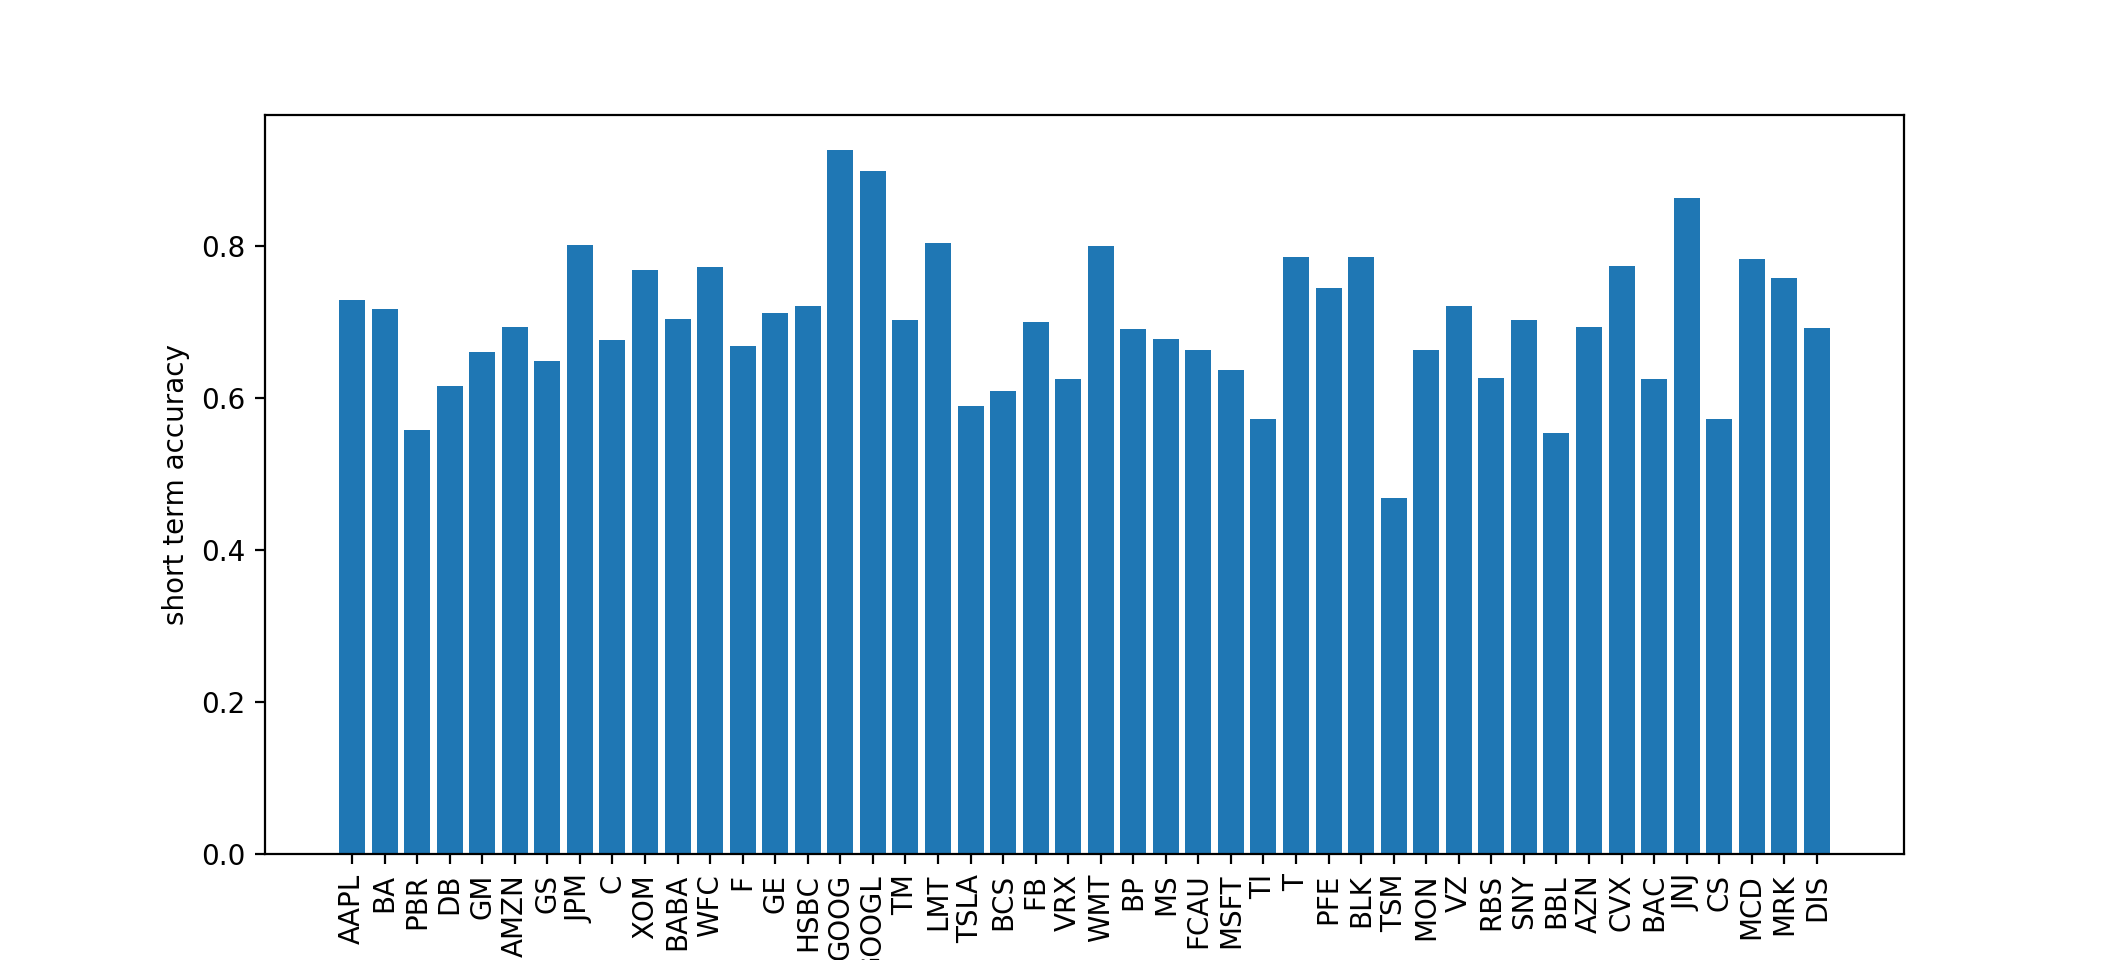
\includegraphics[width=\linewidth]{short-acc.png}
    \caption{各股票短期预测准确率}
    \label{fig:short-acc}
\end{figure}
\begin{figure}[H]
    \centering 
    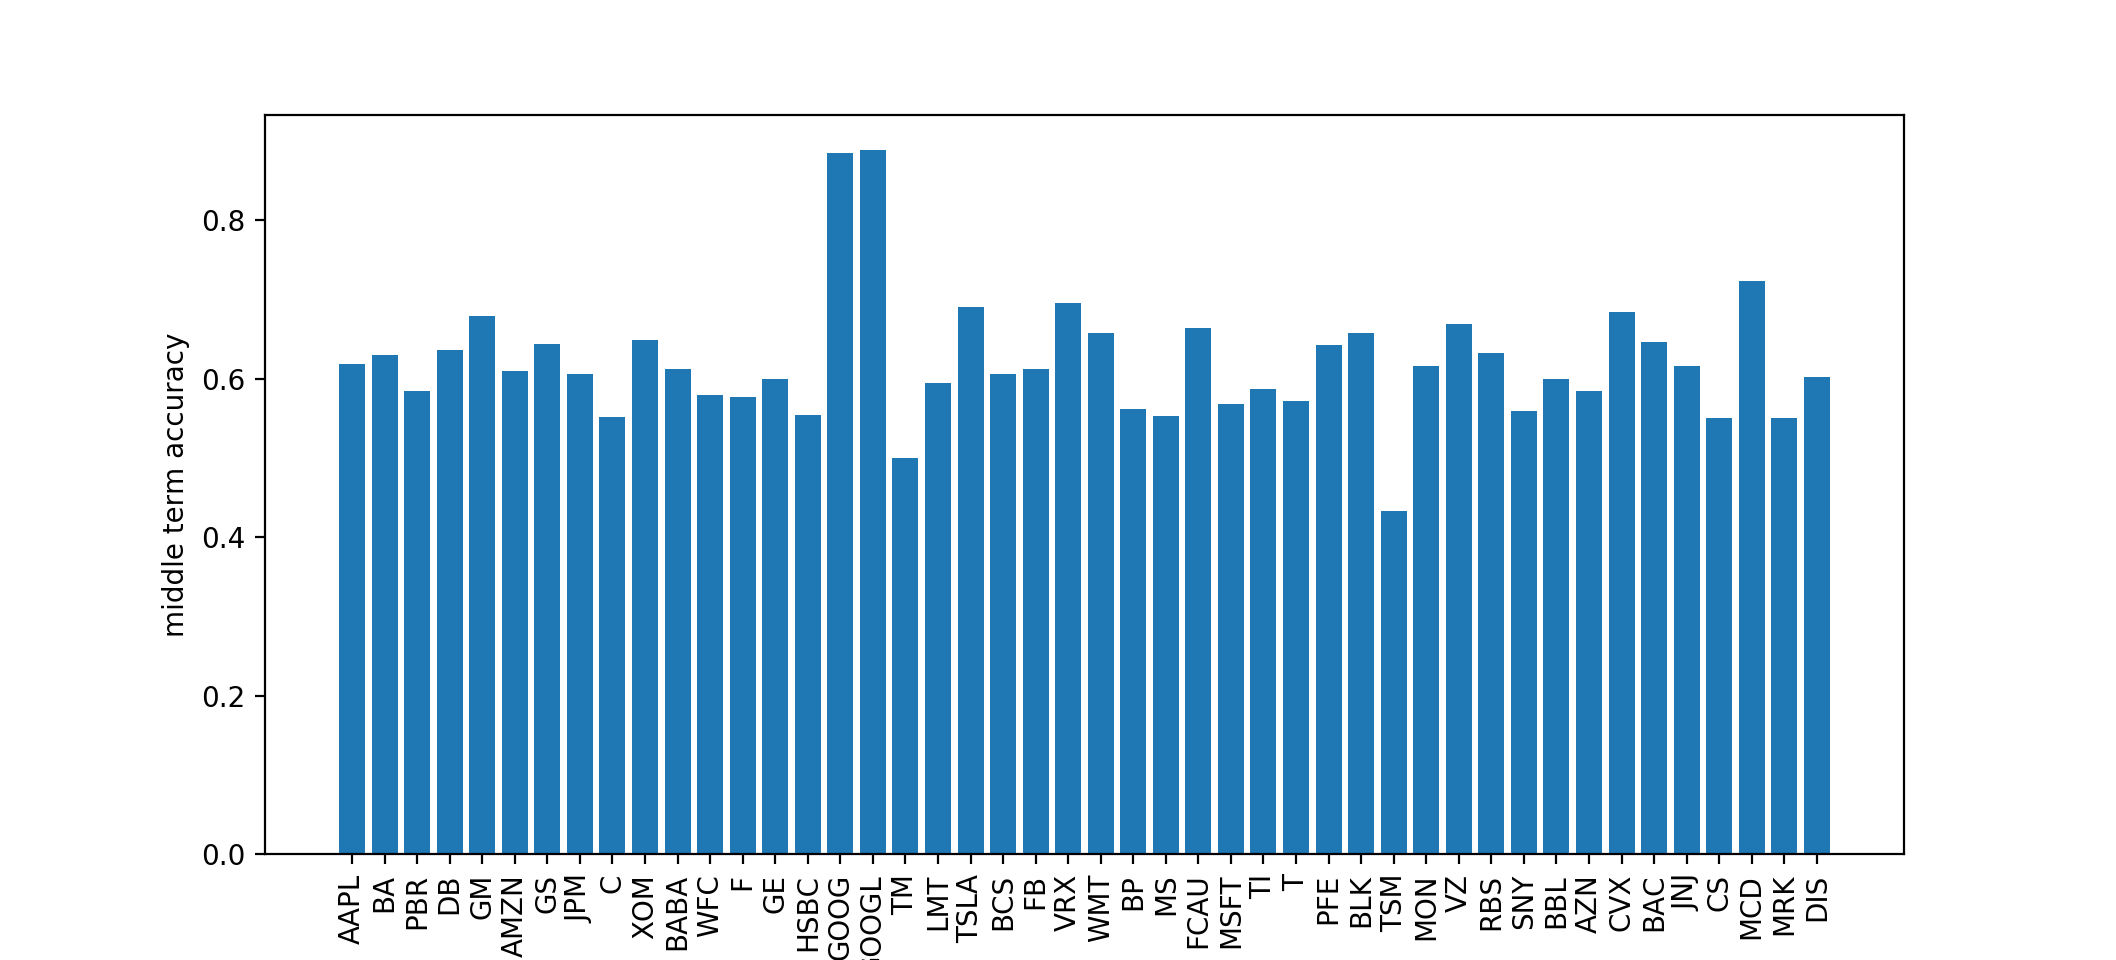
\includegraphics[width=\linewidth]{middle-acc.png}
    \caption{各股票中期预测准确率}
    \label{fig:middle-acc}
\end{figure}
\begin{figure}[H]
    \centering 
    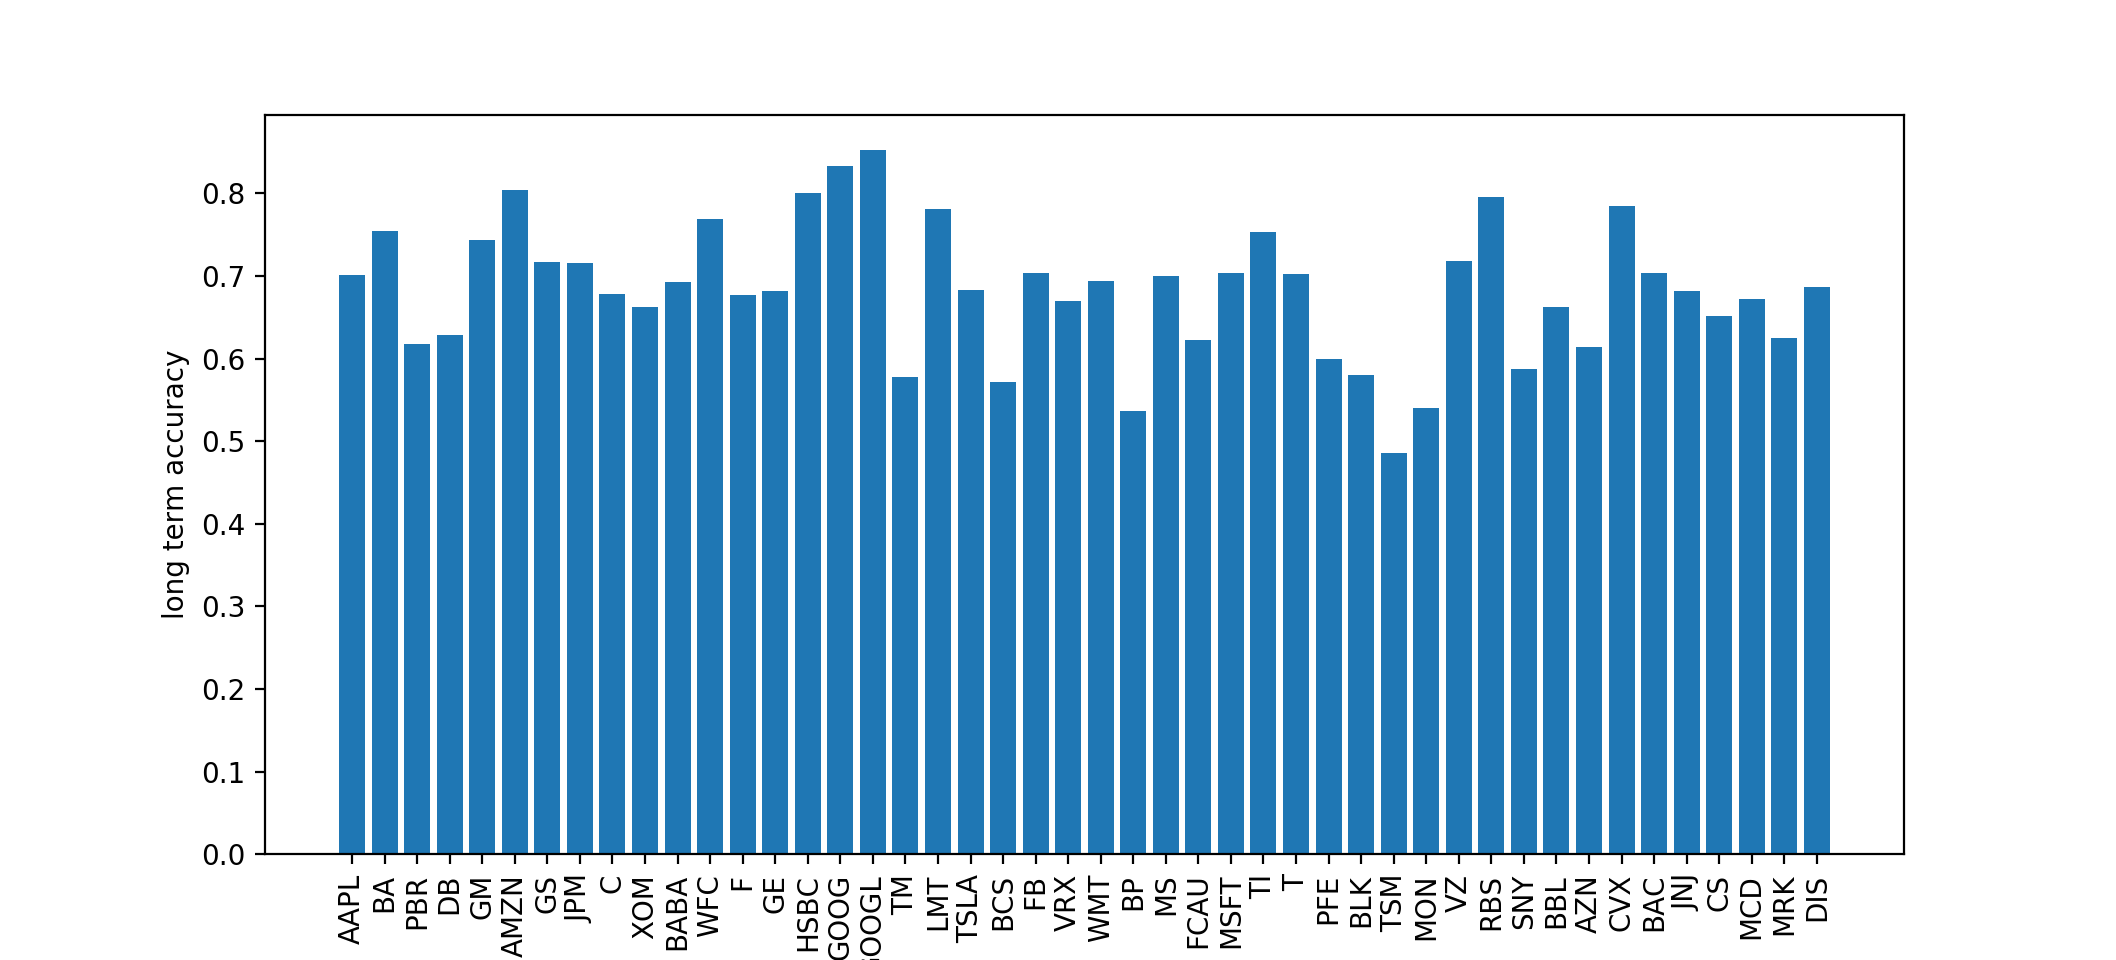
\includegraphics[width=\linewidth]{long-acc.png}
    \caption{各股票长期预测准确率}
    \label{fig:long-acc}
\end{figure}
图\ref{fig:short-acc}、图\ref{fig:middle-acc}、图\ref{fig:long-acc}分别显示了各支股票的短期、中期、长期的预测准确率。短期预测和长期预测的准确率明显比中期预测要高,大部分股票的短期和长期预测准确率均超过了百分之五十。而中期预测的准确率相对较低,大部分股票的中期预测准确率超过了百分之四十。谷歌(GOOG)在短期、中期和长期的预测准确率均超过了百分之八十,说明谷歌的股票价格与其相关新闻关系非常密切。
\subsection{模型简化实验}

\begin{table}[ht]
    \centering
    \caption{模型简化实验结果}
    \label{tab:ablation}
    \begin{tabular}{lcccccc}
    \hlinewd{1.5pt}
    \multirow{2}{*}{Models} & \multicolumn{2}{c}{Short}         & \multicolumn{2}{c}{Middle}        & \multicolumn{2}{c}{Long}                                \\ \cline{2-7} 
                            & Accuracy        & Macro-F1        & Accuracy        & Macro-F1        & Accuracy                   & Macro-F1                   \\ \hline
    CNN                     & 0.6498          & 0.5786          & 0.5813          & 0.5761          & \multicolumn{1}{c}{0.6490} & \multicolumn{1}{c}{0.5961} \\
    MCNN                    & 0.6616          & 0.5852          & 0.5920          & 0.5871          & \multicolumn{1}{c}{0.6531} & \multicolumn{1}{c}{0.6005} \\
    MCSC                    & \textbf{0.6955} & \textbf{0.6208} & 0.6236          & 0.6205          & 0.6765                            & 0.6275                     \\ 
    MSRMAM                    & 0.6920          & 0.6198          & \textbf{0.6273} & \textbf{0.6237} & \textbf{0.6826}                   & \textbf{0.6387}            \\ \hlinewd{1.5pt}
    \end{tabular}
\end{table}
为了证明MSRMAM模型各个部分的有效性,我们进行了模型简化实验。CNN是一个基本的卷积神经网络模型,它只考虑新闻句子的输入,不考虑股票的信息。MCNN使用了多尺度卷积,可以提取不同长度的短语的信息。MCSC使用了股票系数,股票系数引入了股票相关信息。MSRMAM是我们的完整模型,它使用了attention机制,学习股票之间的相关关系。从表~\ref{tab:ablation}可以看到,多尺度卷积和股票系数都可以明显地提升模型的性能。股票关系模型对中期和长期的预测有更大的作用。一种可能的解释是,股票关系模型反映了股票之间的相互关系,这些股票关系与基本面分析更加相关,在中长期的股票价格变动中能展现较大的作用;但在短期预测中,股票价格变化时效性更强,股票关系影响较小。

\subsection{样例分析}

\begin{table}
    \centering  
    \caption{新闻驱动的股票预测样例分析}
    \label{tab:stockcase}
    \begin{tabular}{m{7cm}lm{1cm}m{1cm}m{1.8cm}}
        \hlinewd{1.5pt}
        news title & stock & ATAE-LSTM & GCAE & MSRMAM \\ \hline 
        Tesla delivers quarterly record of 25000 vehicles in first quarter & TSLA\textsubscript{+1} & +1\textsuperscript{\cmark} & -1\textsuperscript{\xmark} & +1\textsuperscript{\cmark} \\  \hline
        Taiwan stocks hit over 18-mth highs TSMC up ahead of Q4 result & TSM\textsubscript{+1} & +1\textsuperscript{\cmark} & 0\textsuperscript{\xmark} & +1\textsuperscript{\cmark} \\ \hline 
        %        Morgan Stanley's profit doubles on bond-trading surge & MS\textsubscript{+1} & -1\textsuperscript{\xmark} & +1\textsuperscript{\cmark} & +1\textsuperscript{\cmark} \\ \hline
        AT\&T to offer hulu to customers this year. & T\textsubscript{+1} & 0\textsuperscript{\xmark} & +1\textsuperscript{\cmark} & +1\textsuperscript{\cmark} \\ \hline
        Consumer reports says Tesla misunderstands 'positive' Model 3 rating & TSLA\textsubscript{-1} & +1\textsuperscript{\xmark} & -1\textsuperscript{\cmark} & -1\textsuperscript{\cmark} \\ \hline
        % Amazon-Apple TV deal shows tough road to cooperation for tech rivals & AMZN\textsubscript{-1} & 0\textsuperscript{\xmark} & -1\textsuperscript{\cmark} & -1\textsuperscript{\cmark} \\ \hline 
        % Apple Google reach new deal with workers xin U.S. lawsuit over hiring & AAPL\textsubscript{+1} & 0\textsuperscript{\xmark} & +1\textsuperscript{\cmark} & +1\textsuperscript{\cmark} \\ \hline
        %        Amazon offers prime discount for U.S. customers on government aid & AMZN\textsubscript{-1} & 0\textsuperscript{\xmark} & 0\textsuperscript{\xmark} & -1\textsuperscript{\cmark} \\ \hline
        % Wal-Mart takes on amazon 's 'prime day ' with online sale & WMT\textsubscript{1} & +1\textsuperscript{\xmark} & +1\textsuperscript{\xmark} & +1\textsuperscript{\xmark} \\ \hline  
        Tesla has recalled 53 000 of its model s model x cars & TSLA\textsubscript{+1} & -1\textsuperscript{\xmark} & -1\textsuperscript{\xmark} & -1\textsuperscript{\xmark} \\ \hlinewd{1.5pt}
    \end{tabular}
\end{table}
为了进一步分析MSRMAM模型的特点,我们在表\ref{tab:stockcase}中展示了新闻驱动的股票预测的样例,正确预测值以下标的形式给出。我们比较了以ATAE-LSTM为代表的LSTM模型和以GCAE为代表了CNN模型,以及我们所提出的股票关系模型。在前两行所展示的例子中,句子都是比较正式,更高的销量或营收可以预测股票价格上涨,LSTM更擅长处理此类问题。在第三行的例子中,因为标题的简洁性,标题与普通句子的语法并不完全一致,CNN能够很好地处理此类问题。第四行中,“misunderstands 'positive' rating”,LSTM误将“positive”识别为积极的消息,CNN模型可以将误解与积极联系成一个短语。另外,在最后一行的例子中,模型预测消息是消极的,从人的主观观察来看,这一结果是正确的,但是,它与股票实际的涨跌不同。我们之前假设股票价格的涨跌仅与前一天、周、月的相关新闻有关,而忽视了其他因素。然而在现实当中,其他因素也发挥着重要作用,新闻并不是决定股票涨跌的唯一因素。为了进一步提升股票预测的准确率,我们可以考虑补充股票历史价格、技术指标等其他信息,这也是后续研究的方向之一。
% \subsection{市场模拟}
% 为了进一步验证我们的模型效果,我们进行了市场模拟实验。我们采用了这样的交易策略\cite{lavrenko2000mining}:我们每天进行一次预测,如果预测某支股票的价格在下一个时间段(天、周、月)内会上涨,则买入价值一万美金的这支股票,如果在下一个时间段内(天、周、月),股票价格上涨超过百分之一,则将其卖出,否则,在下一天、周或月后,将股票卖出;如果预测某支股票价格在下一个时间段(天、周、月)内会下跌,则买空一万美金的这支股票,如果在下一个时间段内(天、周、月),股票价格下跌超过百分之一,则将其卖空,否则,在下一天、周或月后,将股票卖空。我们将初始资金设为三万美金,并利用历史数据进行训练和模拟。我们将购买标普500指数并持有作为基准策略,无风险收益定为百分之三。

% \subsection{策略风险评价指标}

% 策略的风险指标能够从各个维度对策略有客观、全面的评估。本文中,我们使用了以下风险评价指标。
% \subsubsection{年化收益率}
% 年化收益率(Annualized Returns)表示投资一年的预期收益率。
% \begin{equation}
%     p_r=(\frac{p_{end}}{p_{start}})^{\frac{250}{n}}-1
% \end{equation}
% 其中,$p_{end}$是策略最终总资产,$p_{start}$是策略初始总资产,$n$是交易日数量。
% \subsubsection{基准年化收益率}
% 基准年化收益率(Benchmark Returns)表示参考标准年化收益率。
% \begin{equation}
%     B_r=(\frac{B_{end}}{B_{start}})^{\frac{250}{n}}-1
% \end{equation}
% 其中,$B_{end}$是基准最终值,$B_{start}$是基准初始值,$n$是交易日数量。
% \subsubsection{贝塔}
% 贝塔(Beta)表示投资的系统性风险,反映了策略对大盘变化的敏感性。例如,一个策略的Beta为1.3,则大盘涨1\%的时候,策略可能涨1.3\%,反之亦然;如果一个策略的Beta为-1.3,说明大盘涨1\%的时候,策略可能跌1.3\%,反之亦然。
% \begin{equation}
%     \beta=\frac{Cov(p_n,B_n)}{\sigma^2_B}
% \end{equation}
% 其中,$p_n$是策略每日收益率,$B_n$是基准每日收益率,$\sigma^2_B$基准每日收益方差,$Cov(p_n,B_n)$是策略和基准每日收益的协方差。
% \subsubsection{阿尔法}
% 投资中面临着系统性风险(即Beta)和非系统性风险(即Alpha)。Alpha是投资者获得与市场波动无关的回报,一般用来度量投资者的投资技艺。例如,投资者获得了12\%的回报,其基准获得了10\%的回报,那么Alpha或者价值增值的部分就是2\%。
% \begin{equation}
%     \alpha=p_r-r_f-\beta(B_r-r_f)
% \end{equation}
% 其中,$p_r$是策略年化收益率,$r_f$是无风险收益率,$B_r$是基准年化收益率。当Alpha大于零时,说明策略相对于风险,获得了超额收益;当Alpha等于零时,说明策略相对于风险,获得了适当收益;当Alpha小于零时,说明策略相对于风险,获得了较少收益。
% \subsubsection{收益波动率}
% 收益波动率(Volatility)用来测量资产的风险性,波动越大代表策略风险越高。
% \begin{equation}
%     \sigma_p=\sqrt{\frac{250}{n}\sum_{t=1}^{n}(p_t-\overline{p_t})^2}
% \end{equation}
% 其中,$n$是交易日数量,$p_t$是策略每日收益率,$\overline{p_t}=\frac{1}{n}\sum_{t=1}^{n}p_t$策略每日平均收益率。
% \subsubsection{夏普比率}
% 夏普比率(Sharpe Ratio)表示每承受一单位总风险,会产生多少的超额报酬,可以同时对策略的收益与风险进行综合考虑。
% \begin{equation}
%     SharpRatio=\frac{p_r-r_f}{\sigma_p}
% \end{equation}
% 其中,$p_r$是策略年化收益率,$r_f$是无风险收益率,$\sigma_p$是策略收益率波动率
% \subsubsection{信息比率}
% 信息比率(Information Ratio)用来衡量单位超额风险带来的超额收益。信息比率越大,说明该策略单位跟踪误差所获得的超额收益越高,因此,信息比率较大的策略的表现要优于信息比率较小的策略。合理的投资目标应该是在承担适度风险下,尽可能追求高信息比率。
% \begin{equation}
%     InformationRatio=\frac{p_r-B_r}{\sigma_t}
% \end{equation}
% 其中,$p_r$是策略年化收益率,$B_r$是基准年化收益率,$\sigma_t$是策略与基准每日收益差值的年化标准差。
% \subsubsection{最大回辙}
% 最大回撤(Max Drawdown)描述策略可能出现的最糟糕的情况。
% \begin{equation}
%     MaxDrawDown_t=max(1-\frac{P_j}{P_i})
% \end{equation}
% $MaxDrawDown_t$为$t$日的最大回撤,$P_i$和$P_j$分别为$i$日和$j$日的策略总资产,其中$t\ge j>i$。

\subsection{风险提示}
利用MSRMAM模型进行新闻驱动的股票预测是对历史经验的总结,存在失效的可能。股市有风险,投资须谨慎。
\chapter{结论}
\label{cha:conclusion}

\section{本文工作总结}

第\ref{cha:introduction}章介绍了研究内容、研究背影以及本文的贡献。本文研究的是新闻驱动的股票预测,即根据新闻事件,来预测股票价格的涨跌。我们为每支股票创建一个股票向量,从而将新闻驱动的股票预测问题转化为了基于方面的情感分析问题(提取句子对某一目标或方面的情感极性)。之前的研究工作使用词典、结构化实体等方式来表示事件,忽略了新闻文本中的大量细节;另外,之前的工作中所用到的数据集大都是不公开的,这给后续工作增加了难度。为解决这些问题,我们利用路透社的新闻和雅虎财经的股票历史数据创建了公开的新闻驱动的股票预测数据集senti-stock,并提出MSRMAM(基于注意力机制的多股票关系模型)。在senti-stock上的实验证明了我们的模型的有效性。

第\ref{cha:relatedwork}章介绍了基于方面的情感分析的相关工作。这些工作主要可以分为注意力(attention)机制、控制门(gate)方法和记忆网络三类。ATAE-LSTM利用attention方法将目标和句子的信息结合起来,提升了LSTM的效果;IAN通过目标对句子的attention和句子对目标的attention进一步提升了效果。BILSTM-ATT-G用目标将句子分为左边、目标和句子三部分,分别用attention方法对三个部分处理,并用gate对三部分的结果加权求和;GCAE利用CNN处理句子,使得模型更加快速,易于并行,另外,该模型使用CNN计算得到的gate,结合了目标和句子的信息。Memnet将问答领域中的memory network引入到了这一领域,将单词向量直接作为memory,每层利用attention方法对memory加权求和;RAM对Memnet进行了改进,用双向LSTM的输出作为memory,引入了位置权重,弥补attention机制无法处理时序信息的缺陷;TNet结合了LSTM和CNN,使用了不同的位置权重和复杂的attention方法。

第\ref{cha:data}章介绍了本文中所用到的数据集,包括开放数据集餐厅(Restaurant)、笔记本电脑(Laptop)、推特(Twitter)和我们所创建的数据集senti-stock。Restaurant和Laptop是SemEval 2014 Task 4中所用到的数据集,由餐厅和笔记本电脑的评论经人工标注而成;Twitter由推特数据经人工标注而成。这三个数据集是在对目标的情感分析中应用最为广泛的数据集。另外,为了解决之前的新闻驱动的股票预测中公开数据集缺乏的问题,我们构建了senti-stock数据集。我们使用scrapy框架,从路透社和雅虎财经上抓取了大量的股票新闻数据和历史数据。我们假设股票的涨跌仅与前一时间段内股票的相关新闻有关,忽略其他因素。根据下一个时间段的涨跌创建标签,新闻文本作为输入句子,股票作为输入的方面(Aspect)。senti-stock数据集可以在我们给出的链接中获得。

第\ref{cha:transformer}章介绍了我们提出的对目标的情感分析的模型。我们使用了转换器transformer结构,它没有使用长短时记忆网络LSTM和卷积神经网络CNN,完全使用自注意力机制self-attention来处理句子信息;转换器transformer由多层结构构成,每层包含自注意力机制self-attention和前向网络。利用转换器transformer构建的语言模型,在大规模语料库上进行预训练后,可以大大提升后续任务的实验效果。我们使用OpenAI提供的GPT模型。我们将句子与目标拼接,从而将对目标的情感分析问题转化为句子对分类问题。一般情况下,仅使用转换器transformer的第一个token的输出作为整个句子的表示,忽视了其他token的有用信息。我们使用深度可分离depthwise separable的多尺度卷积神经网络CNN,结合了全部的信息,并且降低了参数的数量。

第\ref{cha: msra}章介绍了我们的新闻驱动的股票预测模型MSRMAM(使用注意力机制的多股票关系模型)。我们的模型包括情感分析模块和股票关系模块两部分。这里,我们用到了股票向量,即为每支股票创建一个向量化的表示。情感分析模块使用多尺度卷积处理句子的信息,利用全连接网络学习得到股票系数,通过乘积的方式,将股票的信息和情感特征结合起来。股票关系模块通过注意力机制学习股票之间的相关关系。

第\ref{cha:experiment}章介绍了我们的实验设置和实验结果。在对目标的情感分析方面,我们的基于转换器和多尺度卷积的模型,在公开数据集Reataurant、Laptop、Twitter上均取得了不错的效果;我们进行了模型简化实验,去掉预训练后,模型效果降低很多,可见预训练使得转换器学到了大量的知识,对模型效果有巨大的影响;去掉多尺度卷积后,模型效果降低约1个百分点,可见多尺度卷积可以利用全部token的信息,能够提升模型的效果。在新闻驱动的股票预测方面,MSRMAM模型在senti-stock数据集上取得了不错的效果。在模型简化实验中,我们分别删除了模型中的多尺度卷积、股票系数、股票关系模块。从模型简化实验的结果来看,多尺度卷积能够提取不同长度的短语的特征,股票系数能够引入股票的相关关系,都能够提升模型的效果。股票关系在短期预测中作用不明显,在中长期预测中效果更显著。

最后,我们对全文的贡献作出总结。本文研究了基于方面的情感分析问题及其在新闻驱动的股票预测中的应用。基于方面的情感分析旨在提取一个句子对某一方面或目标的情感极性。我们提出了使用转换器和多尺度卷积的模型来解决对某一目标的情感分析问题,并在公开数据集Restaurant、Laptop、Twitter上取得了不错的结果。同时,我们将基于方面的情感分析应用于新闻驱动的股票预测。通过为每个股票创建一个向量化的表示,我们将新闻驱动的股票预测转化为对某一方面的情感分析问题。我们创建了名为senti-stock的数据集,这一数据集由来自于路透社的金融新闻和雅虎财经的股票历史数据构成,共包括三万条数据。我们提出MSRMAM(多股票关系模型),使用带有股票系数的多尺度卷积提取情感信息,利用注意力机制学习股票之间的相关关系。在senti-stock数据集上的实验证明了模型的有效性。

\section{未来研究展望}

股票预测一直是学术界和金融界的研究热点之一。本文,我们关注于新闻驱动的股票预测,即通过分析新闻,来预测股票的涨跌。通过为每支股票创建一个向量的方式,我们将新闻驱动的股票预测转化为了基于方面的情感分析问题,即预测句子(新闻文本)对方面(股票)或目标的情感极性(涨跌)。为了应对之前研究中新闻表示方法忽视大量细节和缺少公开数据集的问题,我们提出了使用注意力机制的多股票关系模型MSRMAM,并创建了公开的新闻驱动股票数据集senti-stock。在senti-stock上的实验证明了模型的有效性。同时,我们也提出基于转换器和多尺度卷积的模型,并在公开的对目标的情感分析数据集上取得了不错的效果。在未来的研究中,我们仍有许多可以改进和提升的地方。

在数据集方面,为构建数据集,我们假设股票的涨跌仅与前一时间段股票的相关新闻有关,而忽视了其他因素。这一假设在现实当中并不一定成立。为应对这一问题,在后续研究中,我们可以考虑引入其他的因素,如股票的历史数据、技术指标、财报等数据和信息。另外,我们的数据集规模虽然已经比之前的基于方面的情感分析数据集提升了一个数量级,但考虑到股票预测的复杂性,我们可以抓取更多的数据,构建更大的数据集,可能会对股票预测效果的提升有很大帮助。

在模型方面,我们除了我们提出的MSRMAM模型之外,也尝试了其他基于LSTM、CNN、转换器的模型,然而实验的效果并不理想。在引入股票历史数据、技术指标、财报等信息后,如何结合这些多模态的信息,将成为新的问题。如何从模型的构建的角度结合多模态信息,可以成为后续研究的重点方向。

%%% 其它部分
\backmatter
%% 本科生要这几个索引,研究生不要。选择性留下。
% 插图索引
\listoffigures
% 表格索引
\listoftables
% 公式索引
\listofequations

%% 参考文献
% 注意:至少需要引用一篇参考文献,否则下面两行可能引起编译错误。
% 如果不需要参考文献,请将下面两行删除或注释掉。
\bibliographystyle{thuthesis-numerical}
\bibliography{ref/refs}

%% 致谢
% 如果使用声明扫描页,将可选参数指定为扫描后的 PDF 文件名,例如:
% \begin{ack}[scan-statement.pdf]
\begin{acknowledgement}
	衷心感谢导师宋斌恒副教授对本人的精心指导。在研究生期间,宋老师在学习和生活上都给了我巨大的帮助,在学术研究中为我指明方向,指引我追求“独立之人格,自由之思想”。感谢深圳研究生院的吴志勇老师和校外的李智老师在百忙之中参与了本文的评审,他们的意见,对我毕业论文的改进有巨大的帮助。
	
	感谢企业导师陈晓军、崔恒斌和郭迪博士。企业导师帮助我学习学术前沿知识,了解企业业务和技术,提升专业技能。
	
	感谢实验室的罗宁奇同学和沈彬同学。在和他们共同的学习和科研当中,我收获很多;在和他们的交流过程中,也激发了我自己的想法。他们认真刻苦的学风,也深深地感染了我。
	
	感谢 \thuthesis 提供的论文模板。
\end{acknowledgement}


% % %% 附录
\begin{appendix}
\chapter{本文中使用的股票列表}
\label{cha:stock-list}

%\title{本文中使用的股票列表}

\begin{table}[ht]
	\centering 
	\caption{本文中使用的股票列表}
	\label{tab:stock-list}
	\begin{tabular}{|l|m{5cm}|l|m{5cm}|}
		\hline 
		symbol & name & symbol & name\\ 
		\hline 
		AAPL & Apple Inc & BA & Boeing Company (The) \\
		PBR & Petroleo Brasileiro SA- Petrobras & DB & Deutsche Bank AG \\
		GM & General Motors Company & AMZN & Amazoncom Inc \\
		GS & Goldman Sachs Group Inc (The) & JPM & J P Morgan Chase \& Co \\
		C & Citigroup Inc & XOM & Exxon Mobil Corporation \\
		BABA & Alibaba Group Holding Limited & WFC & Wells Fargo \& Company \\
		F & Ford Motor Company & GE & General Electric Company \\
		HSBC & HSBC Holdings plc & GOOG & Alphabet Inc \\
		GOOGL & Alphabet Inc & TM & Toyota Motor Corp Ltd Ord \\
		LMT & Lockheed Martin Corporation & TSLA & Tesla Inc  \\
		BCS & Barclays PLC & FB & Facebook Inc \\
		VRX & Valeant Pharmaceuticals International Inc & WMT & Wal-Mart Stores Inc \\
		BP & BP plc & MS & Morgan Stanley \\
		FCAU & Fiat Chrysler Automobiles NV & MSFT & Microsoft Corporation \\
		TI & Telecom Italia SPA & T & AT\&T Inc \\
		PFE & Pfizer Inc & BLK & BlackRock Inc \\
		TSM & Taiwan Semiconductor Manufacturing Company Ltd & MON & Monsanto Company \\
		VZ & Verizon Communications Inc & RBS & Royal Bank Scotland plc (The) \\
		SNY & Sanofi & BBL & BHP Billiton plc \\
		AZN & Astrazeneca PLC & CVX & Chevron Corporation \\
		BAC & Bank of America Corporation & JNJ & Johnson \& Johnson \\
		CS & Credit Suisse Group & MCD & McDonald\&s Corporation \\
		MRK & Merck \& Company Inc & DIS & Walt Disney Company (The) \\
		\hline 
	\end{tabular}
\end{table}
\end{appendix}

% %% 个人简历
\begin{resume}

  \resumeitem{个人简历}

  1993年5月7日出生于河北省衡水市深县。

  2012年9月考入车辆工程系,2013年7月转入计算机科学与技术系,2016年7月本科毕业并获得工学学士学位。

  2016年9月免试进入清华大学计算机科学与技术系攻读工学学位至今。

  \researchitem{学术论文} % 发表的和录用的合在一起

  % 1. 已经刊载的学术论文(本人是第一作者,或者导师为第一作者本人是第二作者)
  \begin{publications}[before=\publicationskip,after=\publicationskip]
    \item Yinxu Pan, Binheng Song, et al. Transformer and Multi-scale CNN for Target-oriented Sentiment Classification[C]//Asia Pacific Web (APWeb) and Web-Age Information Management (WAIM) Joint Conference on Web and Big Data(APWeb-WAIM) 2019.Chengdu,China.Springer,2019, (CCF-C类会议, 己录用)
    \item Yinxu Pan, Binheng Song, et al. MSRA: Multi-Stock Relation model using Attention mechanism for News-driven Stock Prediction[C]//28th International Conference on Artificial Neural Networks (ICANN).Munich,German:Springer,2019, (CCF-C类会议,己录用)
    \item Ningqi Luo, Binheng Song, Yinxu Pan, et al. Bcmlp: Binary-connected multiplayer perceptrons[C]//The 25th International Conference on Neural Information Processing (ICONIP). Siem Reap, Cambodia: Springer, 2018:77-88. (CCF-C类会议,EI检索,索引号20185206311203)
  \end{publications}

  % % 2. 尚未刊载,但已经接到正式录用函的学术论文(本人为第一作者,或者
  % %    导师为第一作者本人是第二作者)。
  % \begin{publications}[before=\publicationskip,after=\publicationskip]
  %   \item Yang Y, Ren T L, Zhu Y P, et al. PMUTs for handwriting recognition. In
  %     press. (已被 Integrated Ferroelectrics 录用. SCI 源刊.)
  % \end{publications}

  % % 3. 其他学术论文。可列出除上述两种情况以外的其他学术论文,但必须是
  % %    已经刊载或者收到正式录用函的论文。
  % \begin{publications}
  %   \item Wu X M, Yang Y, Cai J, et al. Measurements of ferroelectric MEMS
  %     microphones. Integrated Ferroelectrics, 2005, 69:417-429. (SCI 收录, 检索号
  %     :896KM)
  % \end{publications}

  \researchitem{实践经历} % 有就写,没有就删除
  \begin{achievements}
    \item 2017年6月至2017年9月,于富途证券公司担任量化平台开发工程师。
    \item 2017年10月至2018年3月,于商汤科技公司担任算法实习。
    \item 2018年6月至2018年11月,于蚂蚁金服(杭州)网络技术有限公司担任实习算法工程师。
    \item 2018年12月至2019年4月,于苹果中国担任实习算法工程师。
  \end{achievements}

\end{resume}

\end{document}
